% !TeX spellcheck = Greek_Caps_English_US
\documentclass[article,a4paper,11.2pt]{memoir}


\usepackage{graphicx}
\usepackage{placeins}
%\usepackage{sidenotes}
%\usepackage[a4paper,left=24.8mm,top=27.4mm,headsep=2\baselineskip,textwidth=107mm,
%					marginparsep=8.2mm,marginparwidth=49.4mm,textheight=49\baselineskip,
%					headheight=\baselineskip]{geometry} % tufte-handout definitions
\usepackage[a4paper,
left=22mm,top=27.4mm,
headsep=2\baselineskip,
textwidth=108mm, %110mm
marginparsep=6.0mm, %4.0mm
marginparwidth=70mm, %70mm
textheight=53\baselineskip,
headheight=\baselineskip]{geometry} % tufte-handout definitions

%=======Fonts and Language [XelateX only]=====
\usepackage{fontspec}
\usepackage{float}
\usepackage{morefloats}
\usepackage{polyglossia}

\setmainlanguage{greek}
\setotherlanguage{english}
\setmainfont{Liberation Serif}
\newfontfamily\greekfont{Liberation Serif}
\newfontfamily\greekfontsf{Liberation Serif}
\newfontfamily\greekfonttt{Liberation Serif}

%====Physics and Maths Symbols=============
\usepackage{amsmath}
\usepackage{amssymb}
\usepackage{xparse}
%\usepackage[arrowdel]{physicsrev} %Physics Packge (Revised)
\usepackage[arrowdel]{physics}
\usepackage[version=3]{mhchem} %Chemistry Symbols
\usepackage{wasysym} %Astronomical Symbols

\usepackage{siunitx} %Units
\usepackage{cancel}
\usepackage{multirow}
%=====Graphics=============
\usepackage{graphicx}
%\usepackage{caption}
\usepackage{lipsum, calc, needspace}
%\usepackage{subcaption}
\usepackage{textcomp}
%\usepackage{tikz}
\usepackage{scrextend}
%============================
\newlength\widthw
\setlength{\widthw}{\textwidth+\marginparsep+\marginparwidth}


\newlength{\fullwidthlen}
\setlength{\fullwidthlen}{\marginparwidth}
\addtolength{\fullwidthlen}{\marginparsep}

\newenvironment{fullwidth}{%
	\begin{adjustwidth*}{\ifthispageodd{-5cm}{-0cm}}{\ifthispageodd{-0cm}{-5cm}}%
	}{%
	\end{adjustwidth*}%
}

%======Other==============
\usepackage{multirow}
\usepackage{booktabs}
\usepackage{latexsym,graphicx}
\usepackage{todonotes}
%\usepackage{xcolor}
%\usepackage[some]{background}
%\usepackage{wrapfig}
%\usepackage{sidecap}
%\usepackage{lscape}
%\usepackage{rotating}
%\usepackage{geometry}

%===Bibliography======================
με μι\usepackage[backend=biber,style=authoryear,citestyle=authoryear]{biblatex}
%\addbibresource{My Library.bib}

%=========Unit Declaration==========
\DeclareSIUnit \cm {\centi\meter}
\newcommand{\sm}{$M_{\odot}$}

\title{Αριθμητικές προσομοιώσεις νεφών σε γαλαξίες}
\author{Παπαχρήστου Μιχάλης}

\numberwithin{equation}{subsection}
\setsecnumdepth{chapter}
\setcounter{secnumdepth}{2}
\counterwithout{section}{chapter}
\newcommand{\tabletodo}[3][]{\begin{minipage}{#2}\todo[inline,#1]{#3}\end{minipage}}

\begin{document}
	
\sisetup{retain-unity-mantissa = false,range-phrase=\texttt{ έως },range-units = single}

	
	\maketitle
	Σε αυτή την εργασία θα προσπαθήσουμε να μελετήσουμε μέσω αριθμητικών εξομοιώσεων τη δυναμική ενός μοριακού νέφους (MC) μέσα στο διαγαλαξιακό μέσο (ISM). Για τις αριθμητικές εξομοιώσεις θα χρησιμοποιήσουμε τον κώδικα PLUTO (%\cite{mignone_pluto:_2007})  ώστε να μελετήσουμε μια όσο το δυνατόν ρεαλιστικότερη απεικόνιση ενός σφαιρικού μοριακού νέφους χτίζοντας την, βήμα βήμα μέσω διαφορετικών φυσικών διεργασιών (Radiative Cooling. Magnetic Fields, Gravity, etc)


\section{Μοριακά Νέφη και διαγαλαξιακός χώρος}
Στον μεσοαστρικό χώρο υπάρχει μια τεράστια ποσότητα ύλης υπό τη μορφή αερίου και σκόνης. Η ύλη αυτή, που μπορούμε να πούμε ότι είναι το πρωτόγεννες καύσιμο στη διαδικασία αστρικής δημιουργίας των γαλαξιών, αποτελείται περίπου κατά 99\% από αέριο και κατά 1\% από σκόνη με τη συνολική της μάζα για το δικό μας γαλαξία να είναι της τάξης των \SI{1e9}{ M_{\odot}}, ενώ η πυκνότητα της κυμαίνεται από \SIrange{1e-4}{1e6}{cm^{-3}}.

\begin{marginfigure}
	\label{fig:21}
	\centering
	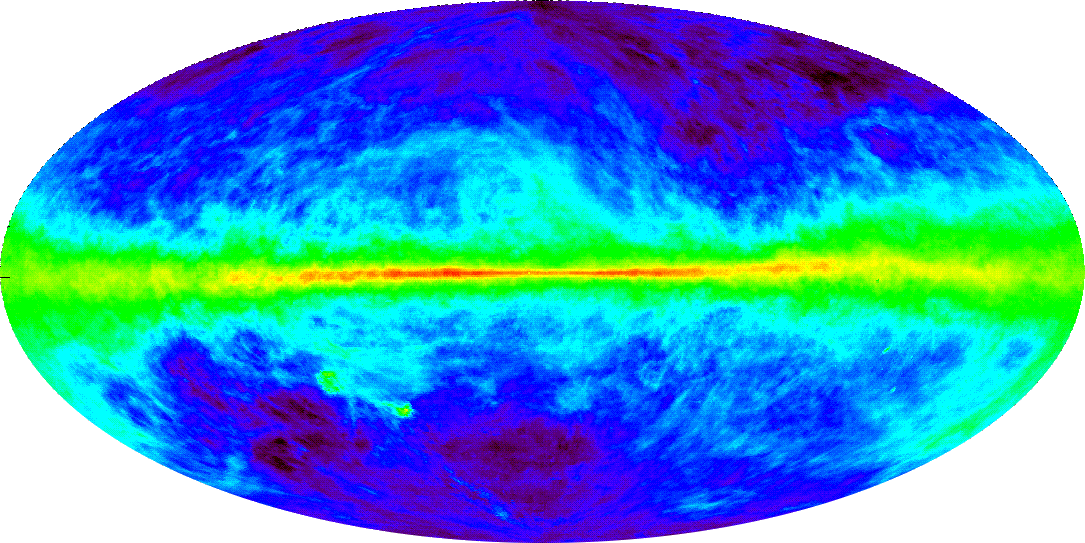
\includegraphics[width=1\linewidth]{Images/21.png}
	\caption{Εκπομπή του \ce{HI} στα 21.1 cm (Kalberla et al., 2005)%\cite{kalberla_2005}.
		H εκπομπή της γραμμής $21.1 \, cm$ στα ραδιοκύματα που οφείλεται στη μετάπτωση αντιστροφής του spin του πρωτονίου και του ηλεκτρονίου στη βασική κατάσταση του ατόμου του Υδρογόνου. Η ενεργειακή διαφορά των καταστάσεων είναι 
		$h \nu=\SI{6e-6}{eV}$, η οποία αντιστοιχεί σε μήκος κύματος \SI{21}{cm}.}
\end{marginfigure}

\begin{marginfigure}
	\label{fig:Ha}
	\centering
	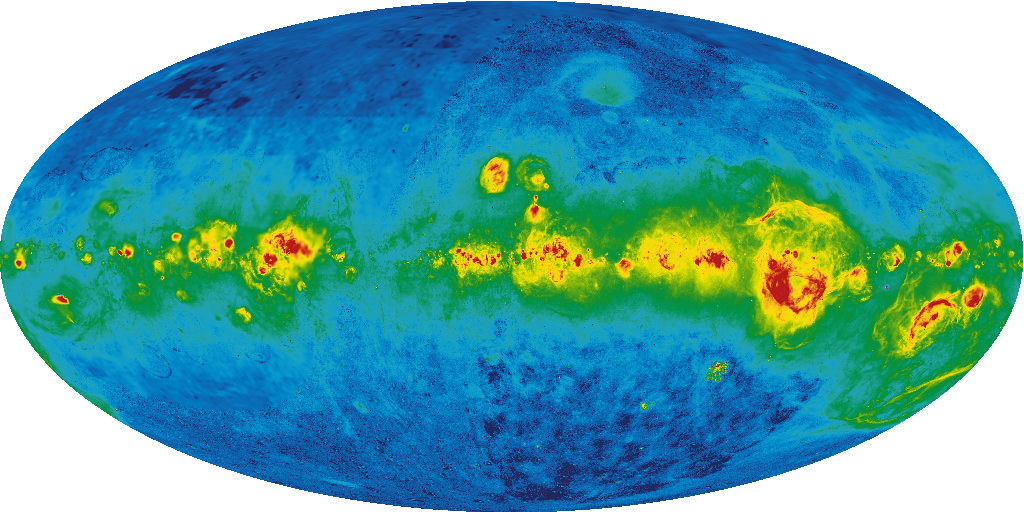
\includegraphics[width=1\linewidth]{Images/Ha.png}
	\caption{Εκπομπή Ha από συνδυασμό τριών διαφορετικών παρατηρήσεων (WHAM - VTSS - SHASSA) \cite{finkbeiner_2003}. Η εκπομπή Ha (\SI{656.28}{nm}) προέρχεται από την επανασύνδεση ιονισμένων ατόμων υδρογόνου κοντά σε θερμούς αστέρες O και B (\ce{HII} Regions).}
\end{marginfigure}


\paragraph{Μεσοαστρικό Αέριο} 
Το Μεσοαστρικό Αέριο παρατηρείται σε νεφελώδη μορφή και αποτελείται κυρίως (περίπου το 90\%) από υδρογόνο σε ατομική \ce{(H)}, ιονισμένη \ce{(HII)} και μοριακή \ce{(H2)} κατάσταση. Δεύτερο σε αναλογία είναι το Ήλιο \ce{(He)} (περίπου 9\%) ενώ το υπόλοιπο 1\% είναι βαρύτερα στοιχεία (\ce{C},\ce{O},\ce{Ne},\ce{Mg},\ce{Fe}, κ.α.) και μόρια (\ce{CO},\ce{CS}, κ.α.).


\paragraph{Μεσοαστρική Σκόνη}
%\begin{figure}[h]
%	\centering
%	\includegraphics[width=\medpage]{images/dust_emission_planck.png}
%	\caption{Εκπομπή της σκόνης του Γαλαξία μας όπως τη χαρτογράφησε το Planck.\cite{planck_2014}}
%\end{figure}

Η Μεσοαστρική Σκόνη αποτελείται κυρίως από άνθρακα και πυρίτιο σε ενώσεις με Υδρογόνο, Οξυγόνο, Μαγνήσιο και Σίδηρο ενώ το μέγεθος των κόκκων της σκόνης κυμαίνεται από \SI{0.01}{\micro\meter} έως \SI{1}{\micro\meter} ακολουθώντας μια κατανομή δύναμης όπου τα μικρότερα μεγέθη είναι πολυπληθέστερα από τα μεγαλύτερα. 
Η Μεσοαστρική Σκόνη παρατηρείται στις σπείρες του Γαλαξία μας (αλλά και σε άλλους γαλαξίες) με τη χαρακτηριστική μορφή τεράστιων σκοτεινών "δρόμων" λόγω της επισκότισης των όπισθεν αστέρων που προκύπτει από την απορρόφηση και σκέδαση του ορατού φωτός.


\section{Φάσεις και χαρακτηριστικά της Μεσοαστρικής Ύλης}
Η Μεσοαστρική Ύλη (ISM) απαντάται σε τρεις φάσεις με διαφορετικά φυσικά και χημικά χαρακτηριστικά: 
\footnote{Για τα χημικά χαρακτηριστικά αναφερόμαστε στή σύνθεση των μορίων και στην αναλογία των στοιχείων. Στα φυσικά χαρακτηριστικά αναφερόμαστε στη πυκνότητα και τη θερμοκρασία της Ύλης} 
τη \textbf{ψυχρή}, με θερμοκρασίες κάτω των \SI{100}{\kelvin},
 πυκνότητα \SIrange{30}{50}{cm^{-3}} και ποσοστό ιονισμού κάτω του 0.1\%, που αποτελείται από μοριακό και ατομικό αέριο Υδρογόνου και σκόνη, τη \textbf{θερμή}, με θερμοκρασίες της τάξης των \SIrange{1e3}{1e4}{K}, πυκνότητες \SI{0.3}{cm^{-3}}, που αποτελείται από ατομικό και ιονισμένο άεριο Υδρογόνο (ποσοστό ιονισμού 2-20\%) και την \textbf{υπέρθερμη} που οφείλεται σε κρουστικά κύματα εκρήξεων supernova και αστρικών ανέμων με θερμοκρασίες τάξης \SI{1e6}{K} και πυκνότητες μικρότερες των \SI{0.01}{cm^{-3}}.

\marginpar{
	\begin{table}[H]
		\caption{Χαρακτηριστικά \newline της μεσοαστρικής ύλης}
		\label{tab:ISM}
		\begin{tabular}{p{2.5cm} c  c  c }
			\toprule
			\multirow{2}{*}{Κατηγορία}  & Θερμοκρασία & Πυκνότητα   \\ 
			& \si{(K)} & \si{(cm^{-1})}  \\
			\midrule
			Μοριακά Νέφη & 10-50 & \num{>1e3} \\
			Ψυχρά Νέφη \ce{HI}  & \num{100} & \num{30} \\
			Θερμό \ce{HI}  & \num{1e3} & \num{0.1} \\
			Θερμό \ce{HII}  & \num{1e4} & \num{1e-2} \\
			Περιοχές \ce{HII} &  \num{1e4} & \num{>100} \\
			Υπέρθερμο Ιονισμένο αέριο &  \numrange{1e6}{1e7} & \num{1e-3} \\
			\bottomrule
		\end{tabular}
	\end{table}
}

\subsection{Ενεργειακή ισορροπία}
\label{par:EnergyBalance}
Η κινητική θερμοκρασία \footnote{Το ψυχρό μεσοαστρικό αέριο λόγω της γενικά χαμηλής του πυκνότητας δεν βρίσκεται σε θερμοδυναμική ισορροπία. Επομένως όταν μιλάμε για θερμοκρασία αναφερόμαστε στη κινητική του θερμοκρασία.\cite[p. 28]{spitzer_1998}} της Μεσοαστρικής Ύλης κυμαίνεται σε ένα εύρος τιμών 6 τάξεων μεγέθους όπως παρατηρούμε και από τον πίνακα~\ref{tab:ISM}. Για να περιγράψουμε και να μοντελοποιήσουμε την ενεργειακή ισορροπία στη Μεσοαστρική Ύλη και άρα να εξηγήσουμε και τις παρατηρούμενες θερμοκρασίες θα πρέπει να υπολογίσουμε τις διαδικασίες θέρμανσης και ψύξης. 
Ενώ η κύρια διαδικασία ψύξης είναι η εκπομπή ακτινοβολίας είτε μέσω αυθόρμητης αποδιέγερσης ή αποδιέγερσης λόγω κρούσης, για τη θέρμανση έχουμε μια πληθώρα διαδικασιών οι οποίες μπορούν να ταξινομηθούν σε 3 κατηγορίες:

\begin{itemize}
	\item θέρμανση από πεδία ακτινοβολίας: φωτοηλεκτρική απορρόφηση σε ουδέτερα στοιχεία, φωτοδιάσπαση στα μόρια, φωτοιονισμός.
	\item θέρμανση μέσω συγκρούσεων: από τυρβώδες ροές, κρουστικά κύματα καταλοίπων supernova και κοσμικής ακτινοβολίας.
	\item θερμική ανταλλαγή μεταξύ της σκόνης και νεφών αερίου, αλληλεπίδραση ιονισμένου αερίου με μαγνητικά πεδία, βαρυτική κατάρρευση. 
\end{itemize}

%\subsection{Παρατηρήσεις της Μεσοαστρικής Ύλης}
%Η παρατήρηση και μελέτη της Μεσοαστρικής Ύλης ποικίλει αναλόγως τη φάση στην οποία βρίσκεται.
%\subparagraph{Εκπομπή 21.1 cm}
%%\begin{figure}[h]
%%	\label{fig:21}
%%	\centering
%%	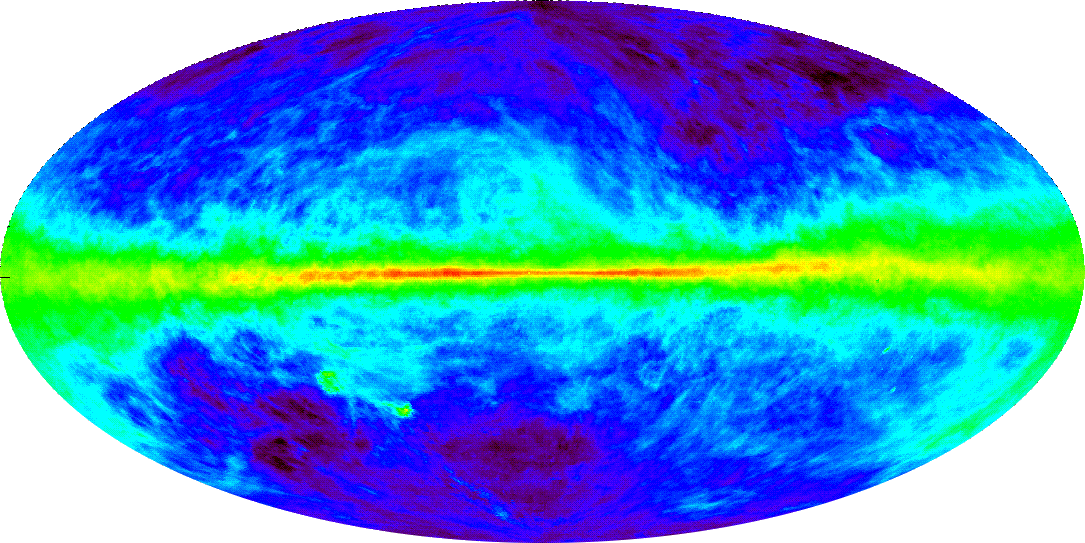
\includegraphics[width=\medpage]{images/21.png}
%%	\caption{Εκπομπή του \ce{HI} στα 21.1 cm (Kalberla et al., 2005)\cite{kalberla_2005}}
%%\end{figure}
%
%H καλύτερη μέχρι σήμερα δυνατή μέθοδος για την παρατήρηση του \textbf{Ουδέτερου Υδρογόνου \ce{H I}} είναι η εκπομπή της γραμμής $21.1 \, cm$ στα ραδιοκύματα που οφείλεται στη μετάπτωση αντιστροφής του spin του πρωτονίου και του ηλεκτρονίου στη βασική κατάσταση του ατόμου του Υδρογόνου. Η ενεργειακή διαφορά των καταστάσεων με συνολικό spin $F=1$ \textbf{(τα spin $p^+$ και $e^-$ είναι παράλληλα)} και $F=0$ \textbf{(τα spin $p^+$ και $e^-$ είναι άντιπαράλληλα)} είναι $h \nu=6\times 10^{-6} \, eV$, η οποία αντιστοιχεί στη γραμμή των 21 cm.
%Ο συντελεστής Einstein για την αυθόρμητη εκπομπή είναι $A_{10} \simeq 3\times 10^{-15}s^{-1}$ που αντιστοιχεί σε μια χρονική κλίμακα των $10^7$ ετών στην οποία παραμένει ένα διεγερμένο άτομο Υδρογόνου μέχρι να αποδιεγερθεί αυθόρμητα εκπέμποντας το παρατηρούμενο φωτόνιο. Ο πολύ μικρός αυτός ρυθμός εκπομπής αντιπαραβάλλεται εν τέλει από τη τεράστια ποσότητα του ατομικού υδρογόνου έτσι ώστε στατιστικά η γραμμή να είναι παρατηρήσιμη.
%
%\subparagraph{Εκπομπή \ce{H\alpha}}
%Κοντά σε αστέρες μεγάλης μάζας (φασματικού τύπου O και B) λόγω των φωτονίων υψηλής ενέργειας (μεγαλύτερες από το όριο Lyman) το αέριο υδρογόνο ιονίζεται. Οι περιοχές αυτές, ονομάζονται και Περιοχές HII, θα τις εξετάσουμε αναλυτικότερα στη παράγραφο~(\ref{par:HII regions}), και παρουσιάζουν έντονη εκπομπή ακτινοβολίας στη γραμμή Ha $(656.28\ nm)$ λόγω της επανασύνδεσης των ιονισμένων ατόμων.

%\begin{figure}[h]
%	\label{fig:Ha}
%	\centering
%	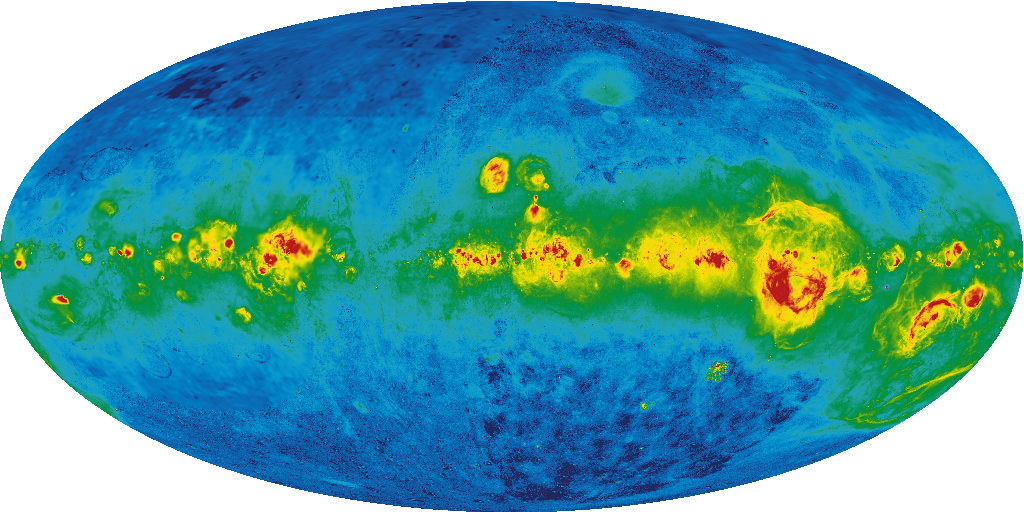
\includegraphics[width=\medpage]{images/Ha.png}
%	\caption{Εκπομπή Ha από συνδυασμό τριών διαφορετικών παρατηρήσεων (WHAM - VTSS - SHASSA) \cite{finkbeiner_2003}}
%\end{figure}
%

%===================================================================
%===================================================================
%===================================================================

\section{Μοριακά Νέφη}
%Οι πιο ενδιαφέρουσες, από τη σκοπιά της δημιουργίας αστέρων, περιοχές του Μεσοαστρικού Υλικού είναι τα Μοριακά Νέφη (Molecular Clouds).
Τα Μοριακά Νέφη είναι περιοχές όπου ψυχρή μεσοαστρική ύλη έχει πυκνότητες ικανοποιητικά μεγαλύτερες από τη μέση πυκνότητα του μεσοαστρικού υλικού έτσι η ιδιοβαρύτητα του νέφους να παίζει σημαντικό ρόλο στη δυναμική του. Καθώς το μοριακό νέφος καταρρέει, κατακρημνίζεται σε όλο και πιο συμπυκνωμένες δομές έως ότου η πυκνότητα και η μάζα σε μια τέτοια περιοχή είναι αρκετή ώστε να γεννηθούν νέοι αστέρες.   

\begin{marginfigure}
	\label{fig:CO}
	\centering
	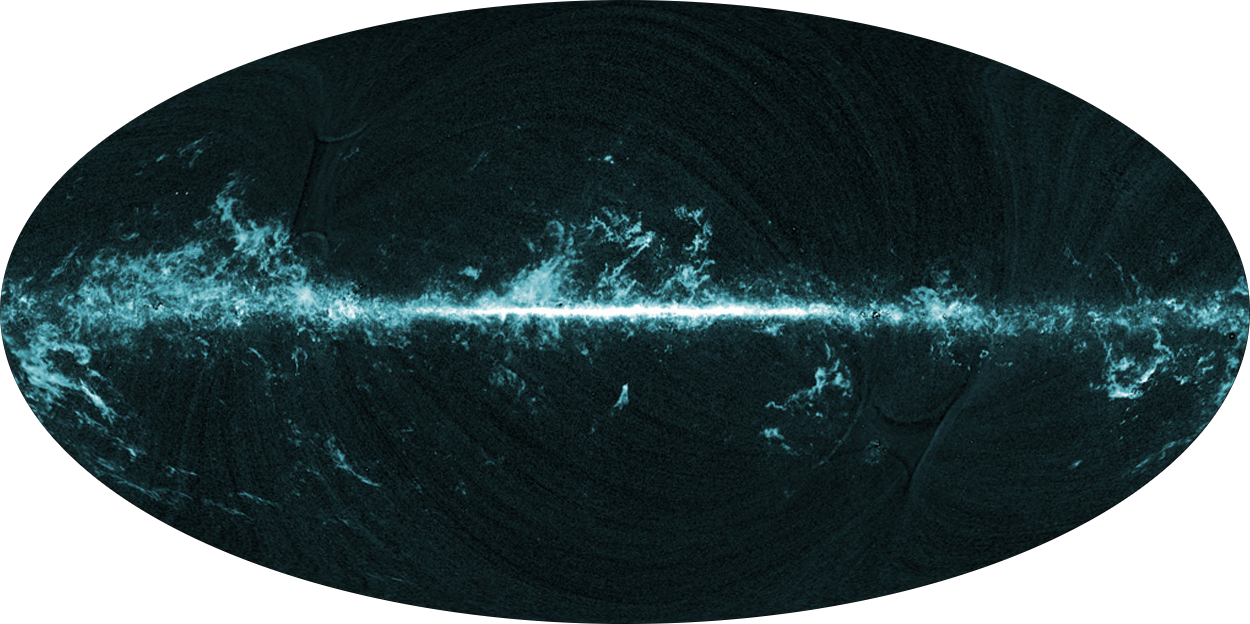
\includegraphics[width=1\linewidth]{Images/CO.png}
	\caption{Εκπομπή CO όπως τη χαρτογράφησε το Planck.\cite{planck_2014}.
		\newline
		Το \ce{H2} είναι ένα πλήρως συμμετρικό μόριο επομένως δεν έχει μόνιμη διπολική ροπή. Αυτό έχει σαν συνέπεια η διέγερση του να είναι σε θερμοκρασίες τις τάξεις των \SI{500}{K}. Άρα για τις τυπικές θερμοκρασίες των μοριακών νεφών $10-50\ K$ είναι αδύνατον να το παρατηρήσουμε άμεσα.
		\newline
		Ο εναλλακτικός τρόπος παρατήρησης του \ce{H2} είναι εμμέσως μέσω της εκπομπής διαφορετικών μορίων που είναι πιο "ευαίσθητα" στις χαμηλές θερμοκρασίες, όπως του \ce{CO} που είναι το δεύτερο σε αναλογία μόριο στο Σύμπαν και έχει μόνιμη διπολική ροπή (άρα έχουμε περιστροφικές ενεργειακές μεταβάσεις) πράγμα του επιτρέπει να εκπέμπει σημαντικά στο ραδιοφωνικό φάσμα.. 
		\newline
		H χαμηλότερη μετάβαση αντιστοιχεί σε θερμοκρασία \SI{5.5}{K} και αποδίδει ένα ραδιοφωνικό φωτόνιο στα \SI{2.6}{mm}.
	}
	%
	%Ο κύριος μηχανισμός διέγερσης ενός μορίου \ce{CO} στη $J=1$ είναι μέσω της σύγκρουσης του με ένα μόριο \ce{H2}. Αφού διεγερθεί η αποδιέγερση του μπορεί να γίνει είτε εκπέμποντας ένα φωτόνιο στα \SI{2.6}{mm} σε περιοχές με χαμηλή συνολική πυκνότητα είτε μεταφέροντας την ενέργεια του σε ξανά σε ένα μόριο \ce{H2} χωρίς να εκπεμφθεί φωτόνιο σε περιοχές με μεγάλη συνολική πυκνότητα.
	
\end{marginfigure}

Όπως φαίνεται και από το όνομα τους, τα Μοριακά Νέφη αποτελούνται κυρίως από μοριακό Υδρογόνο \ce{H2}. Στο γαλαξία μας πάνω από το 80\% του μοριακού Υδρογόνου βρίσκεται σε μοριακά νέφη κατανεμημένα πάνω στις σπείρες του δίσκου αλλά κυρίως σε ένα δακτύλιο ακτίνας 3 με 5 kpc από το κέντρο του γαλαξία \cite{rathborne_2009}.  Από παρατηρήσεις στο \ce{CO} τα μοριακά νέφη δείχνουν να έχουν μάζες που κυμαίνονται από \SIrange{1e3}{1e6}{M_\odot} με μια κατανομή νόμου δύναμης $-1.6$. \cite{stahlern_2004}

Για να δημιουργηθεί το Μοριακό Υδρογόνο καταλυτικό ρόλο παίζει η μεσοαστρική σκόνη.  Όταν δύο άτομα Υδρογόνου ενώνονται και δημιουργούν ένα μόριο \ce{H2} αυτό κερδίζει ενέργεια η οποία όμως δεν μπορεί να αποδοθεί στο περιβάλλον με αποτέλεσμα το μόριο να διασπάται. Παρολαυτά αν η διαδικασία αυτή γίνει πάνω σε έναν κόκκο σκόνης, τότε αυτός λειτουργεί καταλυτικά απορροφώντας το πλεόνασμα ενέργειας και το μόριο παραμένει σταθερό. Έτσι το ουδέτερο Υδρογόνο λειτουργεί σαν καύσιμο που τροφοδοτεί τις πυκνότερες περιοχές του μοριακού Υδρογόνου.

Ένα τυπικό μοριακό νέφος επιβιώνει για \SI{3e7}{yrs} πριν καταστραφεί από τους βίαιους αστρικούς ανέμους των αστέρων τύπου O και B που έχουν δημιουργηθεί στο εσωτερικό του. Κατά τη διάρκεια της ζωής του το νέφος αποδίδει τελικά ένα 3\% της μάζας του σε αστέρες. Έτσι για παράδειγμα αν θεωρήσουμε μια τιμή της συνολικής μάζας του μοριακού \ce{H2} στο Γαλαξιακό δίσκο \SI{2e9}{M_\odot} βρίσκουμε ότι ο ρυθμός δημιουργίας αστέρων (SFR) για το Γαλαξία μας είναι περίπου \SI{2}{M_\odot} ανά έτος.  

\subsection{Ενεργειακή ισορροπία στα Μοριακά Νέφη}
Όπως αναφέραμε γενικότερα στη παράγραφο~(\ref{par:EnergyBalance}) η θερμοκρασία ενός νέφους είναι αποτέλεσμα στης ενεργειακής ισορροπίας μεταξύ των μηχανισμών θέρμανσης και ψύξης. Για τα Μοριακά Νέφη συγκεκριμένα η θέρμανση είναι αποτέλεσμα της θερμότητας που παρέχεται από κοντινά άστρα ή μέσω της κοσμικής ακτινοβολίας, ενώ η ψύξη επιτυγχάνεται μέσω διαδικασιών απορρόφησης και κρούσης με τα σωματίδια της σκόνης ή του αερίου.
Η ενέργεια τελικά αποδίδεται μέσω της υπέρυθρης ακτινοβολίας η οποία οφείλεται στην απορρόφηση και την εκπομπή των φωτονίων από το περιβάλλοντα αέριο και σκόνη.


\begin{table}
	\caption{Χαρακτηριστικά και διαφορετικοί τύποι Μοριακών Νεφών}
	\label{tab:MCtypes}
	\begin{tabular}{l c c c c}
		\toprule
		\multirow{2}{*}{Κατηγορία} & Μέση ακτίνα &  Θερμοκρασία & Πυκνότητα \ce{H2} & Μάζα \\ 
		& \si{(pc)} & \si{(K)} & \si{(cm^{-3})} & \si{(M_\odot)} \\
		\midrule
		Γιγαντιαίο Μοριακό Νέφος & \num{20} & \num{15} & \num{100} & \num{1e5} \\
		Μοριακό Νέφος & $5$ & $10$ & $300$ & $10^4$\\
		clump & $2$ & $10$ & $10^3$ & $10^3$\\
		Πυρήνας Νέφους & $0.08$ & $10$ & $10^5$ & $10$\\
		\bottomrule
	\end{tabular}
\end{table}

\section{Αριθμητικές Μαγνητοϋδροδυναμικές εξομοιώσεις}
Η επίλυση ενός υδροδυναμικού προβλήματος με αριθμητικές μεθόδους είναι μια δύσκολή και πολύ απαιτητική διαδικασία. \todo{αναπτυξε το}

\subsection{Εξισώσεις Διατήρησης}
Οι εξισώσεις διατήρησης είναι χρονοεξαρτώμενα συστήματα μερικών διαφορικών εξισώσεων που έχουν τη γενική μορφή:
\begin{equation}
\label{eq:hyperbolicconservation}
\pdv{t} q(x,t) + \pdv{x} f(q(x,t)) = 0 
\end{equation}
με $q(x,t) \in \mathbb{R}^m$ ένα m-διάστατο άνυσμα των διατηρουμένων ποσοτήτων με  $\int_{-\infty}^{\infty} q_j (x,t) dx$ να είναι η ολική ποσότητα η οποία παραμένει σταθερή στο χρόνο t. 

Η $q(x,t)$ είναι ουσιαστικά η χωρική κατανομή (πυκνότητα) στο χρόνο $t$ η οποία γενικά μεταβάλλεται με το χρόνο.
Αυτή η μεταβολή περιγράφεται από τη συνάρτηση ροής $f_j(q(x,t))$. 
 
Το σύστημα \ref{eq:hyperbolicconservation} είναι η γενικότερη (μη γραμμική) μορφή των γραμμικών υπερβολικών εξισώσεων 
\begin{equation}
\label{eq:linearhyperbolic}
\pdv{q}{t} +  \mathbf{A}\pdv{q}{x}  = 0 
\end{equation}
όπου $\mathbf{A}$ ένας τετραγωνικός διαγωνοποιήσιμος πίνακας με πραγματικές ιδιοτιμές.

Όπως και για τη μονοδιάστατη \todo{Λαθος} περίπτωση 
\begin{equation}
\label{eq:simple_advection}
\pdv{q}{t} +  u\pdv{q}{x}  = 0 
\end{equation}
η οποία έχει σαν λύση τη κυματική λύση D'Alembert
\begin{equation}
q(x,t)=q(x-ut,0)
\end{equation}
η γενική εξίσωση \ref{eq:linearhyperbolic} επιδέχεται αντίστοιχες κυματικές λύσεις.

Στη μη-γραμμική περίπτωση \ref{eq:hyperbolicconservation} το σύστημα λέγεται υπερβολικό αν ο ιακωβιανός πίνακας $\mathbf{J}(q)$ με στοιχεία $(i,j)$ τα $\pdv{f_i}{g_j}$ είναι αντίστοιχα διαγωνοποιήσιμος με πραγματικές ιδιοτιμές.

Τότε μπορούμε να αναζητήσουμε κυματικές αν γραμμικοποιήσουμε το σύστημα γύρω από μια κατάσταση $q_0$ ώστε $q=q_0+\tilde{q}$ ώστε η διαταραχή $\tilde{q}$ να υπακούει στην εξίσωση:
\begin{equation}
\pdv{\tilde{q}}{t} + \mathbf{J}(q_0) \pdv{\tilde{q}}{x} = 0 
\end{equation}

\subsection{Εξισώσεις Euler}
Οι εξισώσεις euler είναι ένα σύστημα μη-γραμμικών υπερβολικών μερικών διαφορικών εξισώσεων που περιγράφουν ένα ρευστό χωρίς ιξώδες και θερμική αγωγιμότητα\marginpar{Τα φαινόμενα διάχυσης (θερμική αγωγιμότητα, μοριακή διάχυση, ιξώδες) δίνουν όρους διάχυσης στη συνάρτηση ροής η οποία τώρα είναι της μορφής $f(q,q_x)$. Αποτέλεσμα αυτού είναι στο δεξί μέλος των εξισώσεων να εμφανίζονται όροι $\pdv*[2]{q}{x}$ και από υπερβολικές να γίνονται παραβολικές. Η πλήρης μορφή των υδροδυναμικών εξισώσεων δίνεται από τις εξισώσεις Navier-Stokes}.   
\begin{align}
&\pdv{\rho}{t} + \div(\rho \vec{u})=0 \label{eq:MassHD} && 
\texttt{Διατήρηση Μάζας} \\
&\pdv{t}(\rho  \vec{u})+\div(\rho  \vec{u}  \vec{u} +P)=0 && 
\texttt{Διατήρηση Ορμής} \label{eq:MomentumHD} \\
&\pdv{E}{t}+\div((E+P)\vec{u})=0 \label{eq:EnergyHD} && 
\texttt{Διατήρηση Ενέργειας}
\end{align}
με $E=\frac{P}{\gamma -1} +\frac{1}{2}\rho u^2$ η ενέργεια για ένα πολυτροπικό αέριο και $P$ η πίεση.

Σύμφωνα με τα προηγούμενα μπορούμε να γράψουμε το σύστημα στη μορφή \ref{eq:hyperbolicconservation}:
\begin{equation}
\pdv{t} \mathbf{q}(\vec{x},t) + \div\mathbf{f}(\mathbf{q}(\vec{x},t)) = 0 
\end{equation}
όπου 
\begin{equation}
\mathbf{q}(\vec{x},t)=\mqty(\rho (\vec{x},t) \\ 
			\rho (\vec{x},t) \vec{u}(\vec{x},t) \\
			E(\vec{x},t))
\end{equation}
και
\begin{equation}
\mathbf{f}(\mathbf{q})= \mqty(\rho \vec{u} \\ 
						\rho \vec{u}\vec{u} + P \\
						\vec{u}(E+P))
\end{equation}

\subsection{Πηγές}
Μέχρι τώρα έχουμε υποθέσει ότι όλες οι διατηρούμενες ποσότητες, "διατηρούνται". Σε πραγματικές συνθήκες όμως υπάρχουν πηγές που προσθέτουν ή αφαιρούν (καταβόθρες) από τις ποσότητες μας. Μερικά παραδείγματα είναι:
\begin{itemize}
	\item Χημικές διεργασίες, ιονισμός και επανασύνδεση που ανταλλάσσουν / δημιουργούν / καταστρέφουν μάζες μεταξύ στοιχείων (διατήρηση της μάζας για πολλαπλά ρευστά)
	\item Εξωτερικές δυνάμεις όπως η βαρύτητα που λειτουργούν σαν πηγές στις εξισώσεις ορμής και ενέργειας.
	\item Μεταφορά θερμότητας μέσω ακτινοβολίας που λειτουργεί σαν πηγή (θέρμανση) ή καταβόθρα (ψύξη)
\end{itemize}
Οι εξισώσεις μας τότε αποκτούν τη μη ομογενή μορφή:
\begin{equation}
\pdv{t} \mathbf{q}(\vec{x},t) + \div\mathbf{f}(\mathbf{q}(\vec{x},t)) = S(\mathbf{q}(\vec{x},t))
\end{equation}

\begin{marginfigure}
	\label{fig:sodleveque}
	\centering
	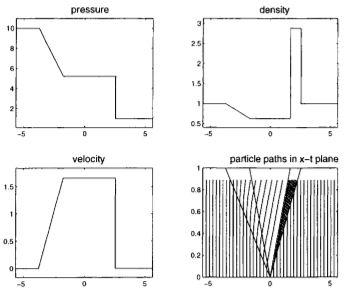
\includegraphics[width=1\linewidth]{Images/SODleveque}
	\caption{Επίλυση του προβλήματος Riemann για τις μονοδιάστατες εξισώσεις Euler με αρχικές συνθήκες όπου η αρχική πίεση στα αριστερά είναι 10πλάσια της αρχικής πίεσης στα δεξιά ενώ οι αρχικές πυκνότητες μένουν ίδιες. Οι χαρακτηριστικές ταχύτητες είναι διαφορετικές (τελευταίο σχήμα) με αποτέλεσμα τα σωματίδια να πυκνώνουν και να δημιουργούν ένα κρουστικό κύμα πύκνωσης προς τα δεξιά, ενώ προς τα αριστερά δημιουργείται ένα κύμα αραίωσης. \cite{leveque_computational_1998}}
\end{marginfigure}
\subsection{Πρόβλημα Riemann}
Το πρόβλημα Riemann είναι η επίλυση ενός νόμου διατήρησης όπως τον έχουμε ορίσει παραπάνω με αρχικές συνθήκες όπου υπάρχει μια ασυνέχεια:
\begin{equation}
\bar{q}(x,0)=
\begin{cases}
\bar{q}_L &\qq{για} x<0 \\
\bar{q}_R &\qq{για} x>0 
\end{cases}
\end{equation}

Όπως βλέπουμε χαρακτηριστικά και στο shock tube problem (\ref{fig:sodleveque}), λόγω της αρχικής ασυνέχειας και της μη-γραμμικότητας των εξισώσεων euler έχουμε σαν αποτέλεσμα τη δημιουργία κρουστικών κυμάτων.


\subsubsection{Γενική επίλυση του γραμμικού προβλήματος Riemann}
Η επίλυση του προβλήματος Riemann στη γραμμική περίπτωση (\ref{eq:linearhyperbolic}) βασίζεται στο μετασχηματισμό των ποσοτήτων $q$ στις λεγόμενες χαρακτηριστικές μεταβλητές $\bar{\xi}=\mathbf{R}^{-1}\bar{q}$ όπου $\mathbf{R}=(\bar{r}_1,\bar{r}_2,\cdots \bar{r}_m)$ ο πίνακας των ιδιοανυσμάτων του πίνακα $\mathbf{A}=\mathbf{R}\mathbf{\Lambda}\mathbf{R}^{-1}$. Με $\bar{\Lambda}=\mathtt{diag}(\lambda _1,\lambda _2,\cdots \lambda _m)$ ο διαγώνιος πίνακας των ιδιοτιμών.

Οι εξισώσεις τότε γράφονται:
\begin{equation}
\pdv{\bar{\xi}}{t} + \bar{\Lambda} \div\bar{\xi} =0
\end{equation} 
δηλαδή σαν ένα διαχωρισμένο σύστημα εξισώσεων της μορφής \ref{eq:simple_advection} με λύσεις:
\begin{equation}
\label{eq:xi_solution}
\xi_p  = \xi_p(x-\lambda _p t,0) 
\end{equation}
με $p=1...m$ για τις $m$ εξισώσεις (μονοδιάστατη περίπτωση). Οι $p$ χαρακτηριστικές καμπύλες δηλαδή καθορίζονται από τις ιδιοτιμές $\lambda _p$.

Άρα αν επιστρέψουμε στις αρχικές μεταβλητές:
\begin{equation}
\bar{q}(x,t) = \sum_{p=1}^{m} \xi_p(x-\lambda _p t,0)\bar{r}_p
\end{equation}

Για τις αρχικές συνθήκες του προβλήματος Riemann o μετασχηματισμός μας δίνει:
\begin{equation}
\xi_p (x,0) =
\begin{cases}
u^L_p &\qq{για} x<0 \\
u^R_p &\qq{για} x>0 
\end{cases}
\end{equation} 

άρα από \ref{eq:xi_solution}
\begin{equation}
\xi_p (x,t) =
\begin{cases}
u^L_p &\qq{για} x-\lambda _p t<0 \\
u^R_p &\qq{για} x-\lambda _p t>0 
\end{cases}
\end{equation} 

\begin{marginfigure}
	\label{fig:linearriemann-leveque}
	\centering
	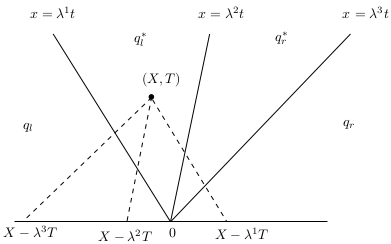
\includegraphics[width=1\linewidth]{Images/LinearRiemann-leveque}
	\caption{Λυση γραμμικου riemann}
\end{marginfigure}

φσαδα 

Άρα με αρχικές συνθήκες Riemann, βλέπουμε ότι η λύση για τις μετασχηματισμένη μεταβλητή $\xi _p$ σε ένα οποιαδήποτε σημείο εξαρτάται απόλυτα αό τη σχετική θέση σε σχέση με την αντίστοιχη χαρακτηριστική καμπύλη της $\lambda _p$.  

Καθώς διασχίζουμε τη καμπύλη αυτή ουσιαστικά μετακινούμαστε από τις συνθήκες $\xi^L_p$ στις $\xi^R_p$. Το άλμα αυτό υπακούει τις συνθήκες Rankine-Hugoniot \todo{Rankine-Hugoniot} άρα για κάθε σημείο μπορούμε τελικά να γράψουμε τη λύση.
\begin{equation}
\bar{q}(x,t)=q_L + \sum_{\lambda_p<x/t} (\xi ^R_P - \xi ^L_P) \bar{r_p}
			=q_R - \sum_{\lambda_p>x/t} (\xi ^R_P - \xi ^L_P) \bar{r_p}
\end{equation}
\todo{Επιλυση γραμμικου Riemann διαγραμμα}

\subsubsection{Επίλυση του μη γραμμικού προβλήματος Riemann}



\subsection{Κώδικας PLUTO}

Ο PLUTO είναι σχεδιασμένος ώστε να ολοκληρώνει ένα γενικό σύστημα νόμων διατήρησης της μορφής:
\begin{equation}
\pdv{\mathbf{U}}{t} = -\div \mathbf{T}(\mathbf{U}) +\mathbf{S}(\mathbf{U})
\end{equation}
όπου $\mathbf{U}$ είναι το άνυσμα των διατηρουμένων ποσοτήτων, $\mathbf{T}(\mathbf{U})$ είναι ένας τανυστής 2ης τάξης με τις ροές των ποσοτήτων και $\mathbf{S}(\mathbf{U})$ οι πηγές/καταβόθρες.

Here U denotes a state vector of conservative quantities, T(U) is a rank-2 tensor, the rows of which are the
fluxes of each component of U and S(U) defines the source terms. Additional source terms may implicitly
arise when taking the divergence of T(U) in a curvilinear system of coordinates. An arbitrary number of
advection equations may be added to the original conservation law (1).

%\begin{equation}
%\label{eq:MassHD}
%\pdv{\rho}{t} + \div(\rho \vec{u})=0
%\end{equation}
%
%\begin{equation}
%\label{eq:MomentumHD}
%\pdv{t}(\rho  \vec{u})+\div(\rho  \vec{u}  \vec{u} +P)=0
%\end{equation}
%
%\begin{equation}
%\label{eq:EnergyHD}
%\pdv{E}{t}+\div((E+P)\vec{u})=S
%\end{equation}


	\section{Ορισμός του Προβλήματος}
	\subsection{Αρχικές Συνθήκες}
	\label{par:InitialConditions}
	Θεωρούμε ένα στατικό μοριακό νέφος ακτίνας $\SI{10} {pc}$ με αριθμητική πυκνότητα
	της τάξης των $\SI{1000}{cm^{-3}}$ δηλαδή πυκνότητας $\rho=\SI{1.67e-21}{g. \cm^{-3}}$ και θερμοκρασίας $T=\SI{100}{\kelvin}$.
	Για το διαγαλαξιακό μέσο θεωρούμε αντίστοιχα μια αριθμητική πυκνότητα της τάξης του 
	$\SI{1}{\cm^{-3}}$ δηλαδή $\rho=\SI{1.67e-24}{g. \cm^{-3}}$ και θερμοκρασία $T=\SI{1e5}{\kelvin}$.

			\begin{marginfigure}
				\centering
				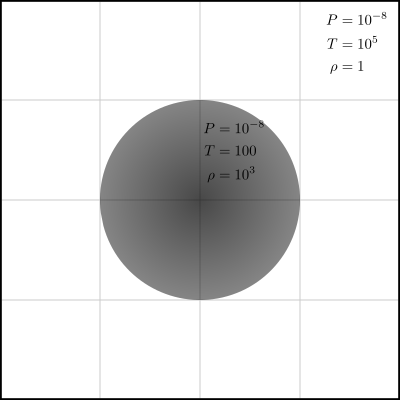
\includegraphics[width=0.7\linewidth]{Images/rect4578.png}
				\caption{Αρχικές συνθήκες ενός στατικού σφαιρικού νέφους ακτίνας \SI{10}{pc}}
				\label{fig:rect4578}
			\end{marginfigure}
		
	\subsection{Μονάδες κώδικα}
	Για την εξομοίωση θα χρησιμοποιήσουμε μονάδες κώδικα \todo{γιατί?}
	
			\begin{table}[H]
				\centering
				\caption{Code Units}
				\label{tab:cd}
				\begin{tabular}{|l|  c |  c|}
					\toprule
					Quantity & Symbol & Code Unit\\ 
					\midrule
					Length & $L_0$ & $\SI{3e19}{\cm} = \SI{10}{pc}$ \\
					Velocity & $V_0$ & $\SI{3e10}{\cm \sec^{-1}}$\\
					Density& $\rho_0$&$\SI{1.67e-24}{g.\cm^3}$\\
					%\multirow{2}{*}{Mass \\ Density} &\multirow{2}{*}{$\rho_0$}  & \multirow{2}{*}{$\SI{1.67e-21}{g. \cm^{-3}}$} \\ \\
					Time & $t_0=\frac{L_0}{V_0}$ & $10^9\si{\sec} =\SI{32}{yrs}$\\
					Pressure & $P_0=\rho_0 V_0^2$ &$\SI{1.5e-3}{dyn.cm^{-2}}$ \\
					Temperature &$T_0=\frac{V_0^2m_p}{k_b}$&$10^{13}\si{\kelvin}$  \\		
					\bottomrule
				\end{tabular}
			\end{table}

%	From the set of $\{L_0,V_0,\rho_0 \}$ we can derive the units of \textbf{time} $t_0=\frac{L_0}{V_0}=10^9\si{\sec}\simeq\SI{32}{yrs}$ 
%	and \textbf{Pressure} $P_0=\rho_0 V_0^2 =\SI{1.5e-3}{dyn}$
	
	
	\section{Σφαιρικό νέφος μέσα στην ISM}
	Αρχικά θα εκτελέσουμε τη προσομοίωση μας χωρίς καμία "ιδιαίτερη" φυσική διεργασία,
	δηλαδή θα αφήσουμε ελεύθερο ένα πυκνό σφαιρικό νέφος με τις παραπάνω αρχικές συνθήκες μέσα στο αραιό-θερμό διαγαλαξιακό αέριο.
	
	\begin{marginfigure}
	%\centering
	\caption{Στιγμιότυπα του νέφους έως τα 8 εκατομμύρια χρόνια.}
	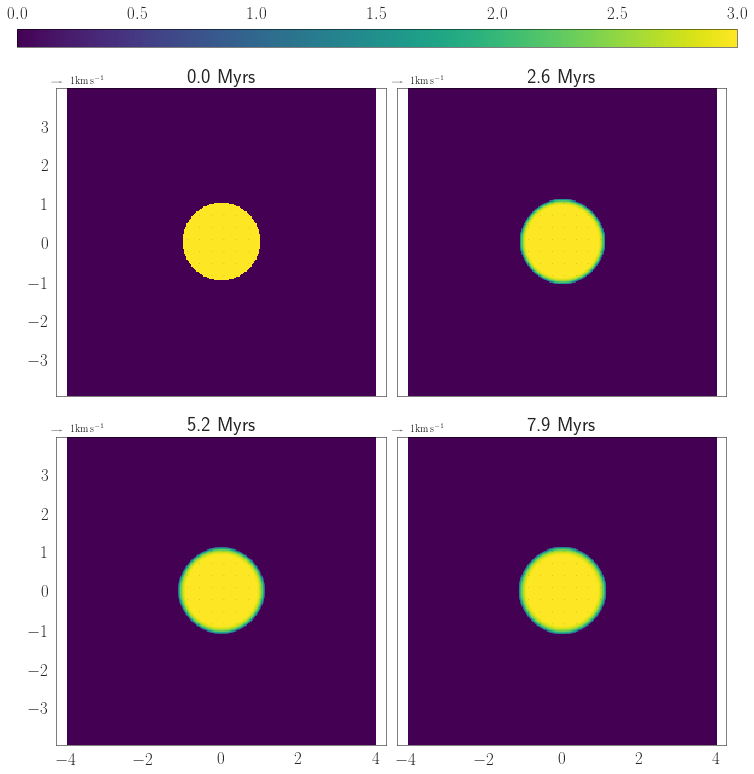
\includegraphics[width=1.0\linewidth]{DataImages/NoCoolingRHOquad.png}
	\label{fig:NoCoolingRHOquad}
	\end{marginfigure}	

 Όπως παρατηρούμε από το σχήμα~\ref{fig:NoCoolingRHOquad} και καλύτερα από το σχήμα~\ref{fig:nocoolingrhoprofile} μέσα σε 8 εκατομμύρια χρόνια το νέφος είναι στη πράξη σταθερό με τη μόνη "δυναμική" που τείνει να διασταλεί το νέφος να είναι η διάχυση, \todo[inline]{Πρόβλημα Riemann, shock?, diffusion rate?} ενώ η πίεση παραμένει παντού σταθερή (το σχήμα παραλείπεται).  
 
 
\begin{figure}[h]
	\centering
	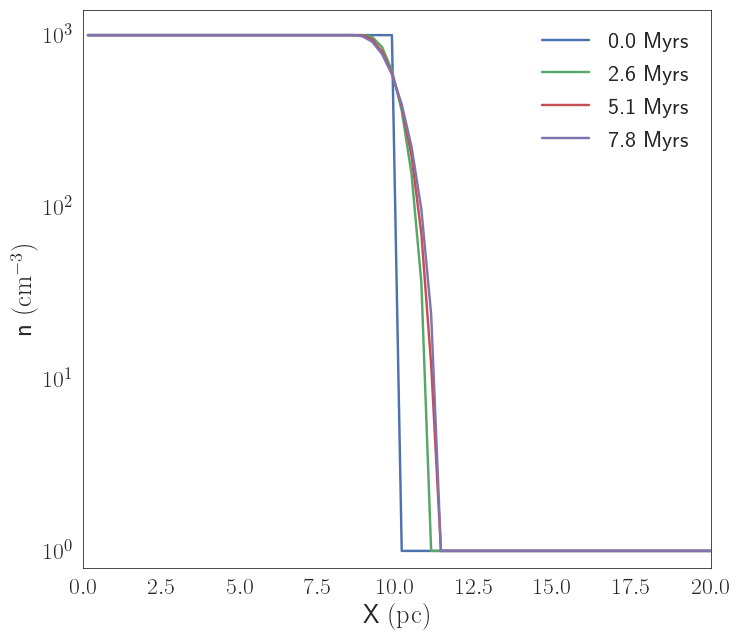
\includegraphics[width=1.0\linewidth]{DataImages/NoCoolingRHOprofile}
	\caption{Προφίλ της πυκνότητας κατά μήκος της ευθείας $y=0$.}
	\label{fig:nocoolingrhoprofile}
\end{figure}
	
	\section{Σφαιρικό νέφος με Radiation Cooling}
		
	Η πρώτη φυσική διεργασία που μας δίνει την ευκαιρία ο PLUTO με τη χρήση διάφορων modules να εξετάσουμε είναι αυτή της Ψύξης μέσω ακτινοβολίας (Radiation Cooling).
	
	\subsection{Γενικά περί Radiation Cooling}
	\todo[inline]{Γενικά περί Radiation Cooling}

	\subsection{Οπτικό βάθος}
	Το νέφος έχει αριθμητική πυκνότητα $\SI{1000}{atoms.cm^{-3}}$ άρα το οπτικό βάθος
	για ένα φωτόνιο που εκπέμπεται μέσα στο νέφος είναι:
	\begin{equation}
	\tau = nL\sigma _T\simeq \num{6.65e-3}
	\end{equation}
	όπου $\sigma _T = \SI{6.65e-25}{cm^2}$ είναι η ενεργός διατομή Thomson.
	
	Έτσι μπορούμε να συμπεράνουμε οτι είναι οπτικά αδιαφανές, άρα η ψύξη θα γίνεται ταυτόχρονα σε όλο τον όγκο του νέφους. 
	
	\subsection{Tabulated Cooling}
	Ο Pluto έχει τη δυνατότητα εξομοίωσης του radiation cooling μέσω της προσθήκης του αντίστοιχου όρου στην εξίσωση 
	της Ενέργειας (\ref{eq:EnergyHD}). Για ένα οπτικά αδιαφανές μέσο δηλαδή: 
	\begin{equation}
		\pdv{t}(\rho e)=-\Lambda^*(n,T)=-n^2 \Lambda(T)
	\end{equation}
	
		\begin{marginfigure}
		%\centering
		\caption{Παράμετρος ψύξης $\Lambda$}
		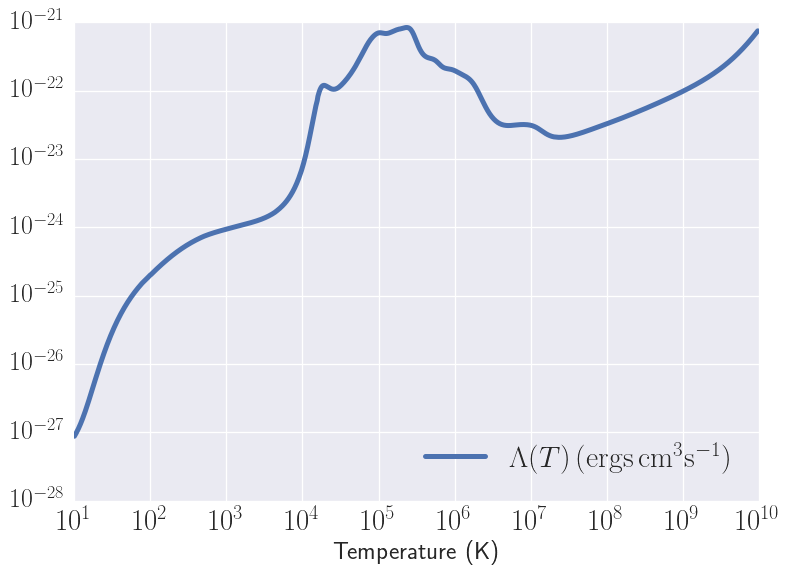
\includegraphics[width=1.0\linewidth]{Images/LambdaT}
		\label{fig:LambdaT}
	\end{marginfigure}

	όπου  $\Lambda (T )$  είναι μια συνάρτηση με αριθμητικές τιμές από έναν εμπειρικό πίνακα. Οι τιμές της συνάρτησης για διαφορετικές θερμοκρασίες φαίνονται στο σχήμα~\ref{fig:LambdaT}) σε μονάδες $ \si{ergs.\cm^3 s^{-1}}$ και για  $n=\frac{\rho}{\mu m_u}$

	
	\subsubsection{Χρονική κλίμακα ψύξης}
	Για μια αρχική θερμοκρασία $T=\SI{100}{K}$ και αριθμητική πυκνότητα $n=10^3\si{protons.cm^{-3}}$ μπορούμε να εκτιμήσουμε τη χρονική κλίμακα ψύξης του νέφους:
	\marginpar{\centering $k_b=\SI{1.38e-16}{ergs.K^{-1}}$}
	\begin{equation}
		\tau _c =\frac{ \rho e} {n^2 \Lambda (T)}=
		\frac{ \frac{3}{2}k_b T} {n \Lambda (T)} 
		\simeq 10^8\si{s}\simeq \SI{3}{yrs}
	\end{equation}
	Βλέπουμε ότι η χρονική κλίμακα ψύξης είναι τάξης ετών, δηλαδή εξαιρετικά μικρή σε σχέση με τους χρόνους που εξομοιώνουμε (τάξης $10^5\si{yrs}$) και τους χρόνους δυναμικής των νεφών γενικά. \todo[inline]{διατύπωση}  
	
	
	\subsubsection{Δυναμική του νέφους}
	Καθώς το αέριο κρυώνει στο εσωτερικό του νέφους η πίεση $P \sim \rho T$ μικραίνει σε αναντιστοιχία με το περιβάλλον αέριο, με αποτέλεσμα να δημιουργείται μια διαφορά πίεσης η οποία θα έπρεπε να επιταχύνει το αέριο προς το εσωτερικό του. Από τις εξομοιώσεις όμως, βλέπε σχήματα (\ref{fig:tabcoolingrhoprofile},\ref{fig:tabcoolingprsprofile-gradp}) παρατηρούμε το αντίθετο αποτέλεσμα, δηλαδή μια διαφορά πίεσης με φορά δύναμης προς τα έξω. 
	
	\begin{marginfigure}
		%\centering
		\caption{Ο χάρτης της πυκνότητας του νέφους στο χρόνο σε λογαριθμική κλίμακα.}
		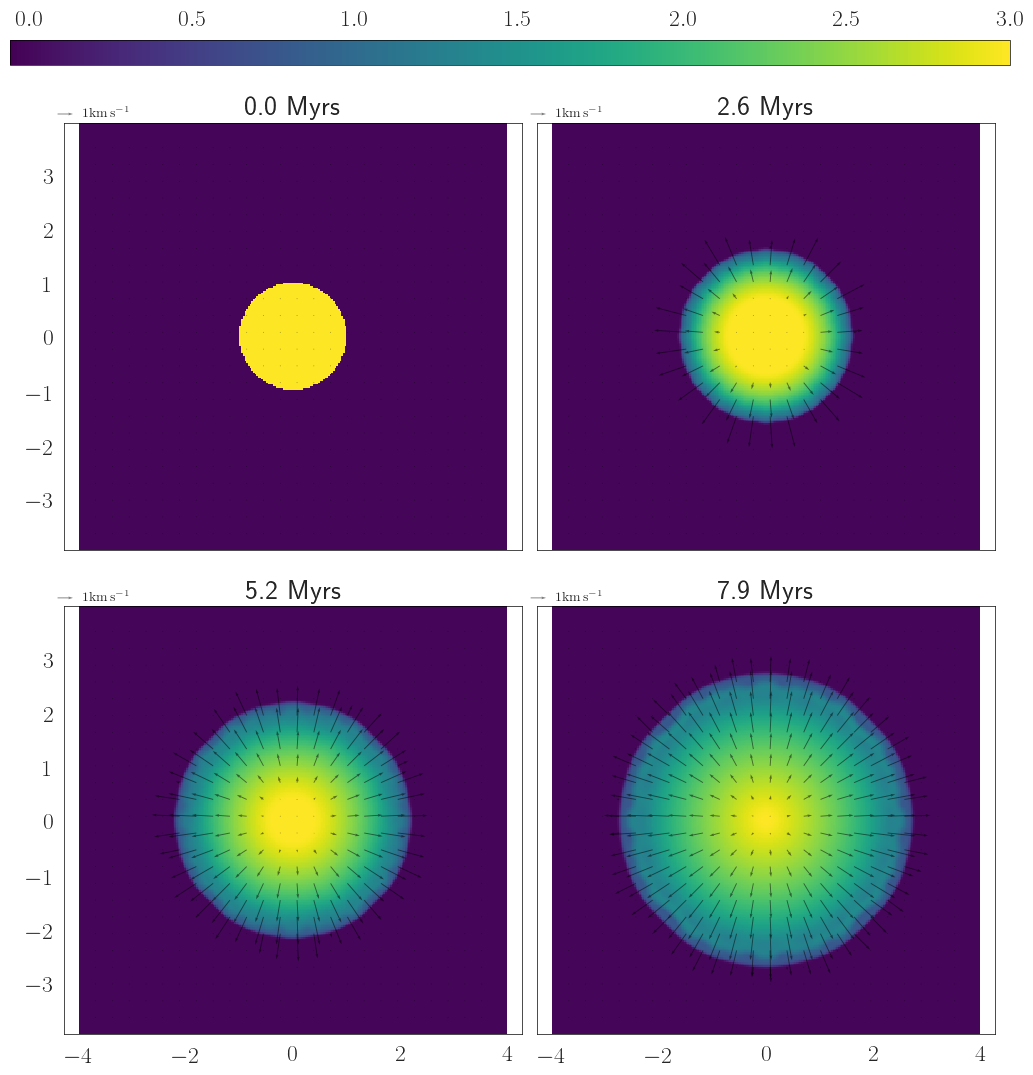
\includegraphics[width=1.0\linewidth]{DataImages/TabCoolingRHOquad}
		\label{fig:TabCoolingRHOquad}
	\end{marginfigure}
	

	\begin{figure}[h]
		\begin{adjustwidth*}{-5cm}{-0cm}%
		\centering
		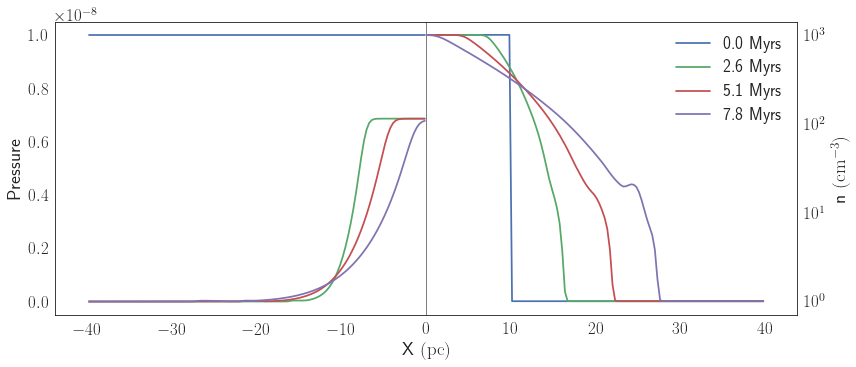
\includegraphics[width=1\linewidth]{DataImages/TabCoolingRHOprofile}
		\caption{Το προφίλ της πυκνότητας του αερίου με ενεργοποιημένο το Tabulated Cooling Module κατά μήκος της ευθείας $y=0$ με το χρόνο.}
		\label{fig:tabcoolingrhoprofile}
		
		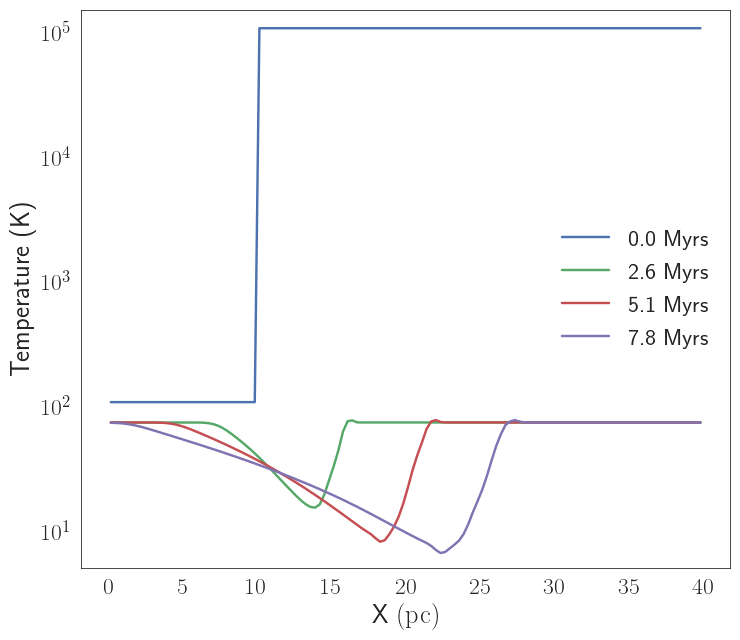
\includegraphics[width=1\linewidth]{DataImages/TabCoolingTMPprofile}
		\caption{Το προφίλ της θερμοκρασίας του αερίου με ενεργοποιημένο το Tabulated Cooling Module κατά μήκος της ευθείας $y=0$ με το χρόνο.}
		\label{fig:tabcoolingtmpprofile}
		
		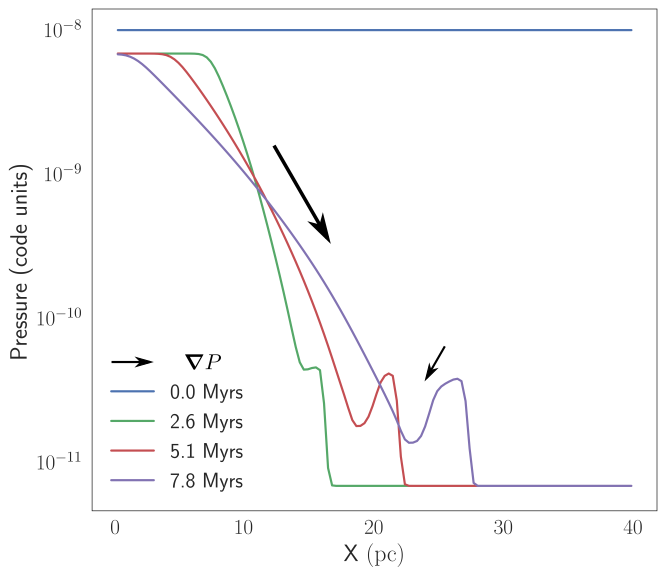
\includegraphics[width=1\linewidth]{DataImages/TabCoolingPRSprofile-gradP}
		\caption{Το προφίλ της πίεσης του αερίου με ενεργοποιημένο το Tabulated Cooling Module κατά μήκος της ευθείας $y=0$ με το χρόνο. Ενδεικτικά (εκτός κλίμακας) δείχνουμε και τη κλίση της πίεσης.}
		\label{fig:tabcoolingprsprofile-gradp}
	\end{adjustwidth*}
	\end{figure}

	
\begin{marginfigure}
	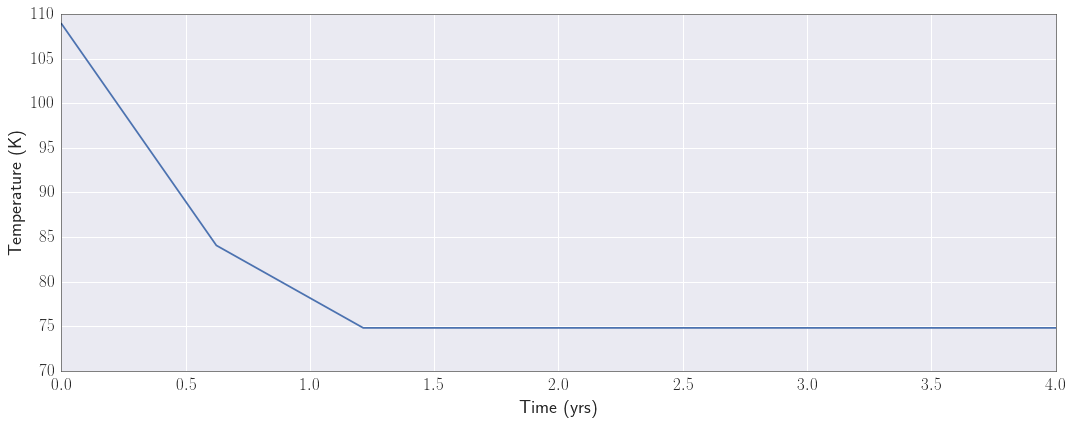
\includegraphics[width=1\linewidth]{DataImages/TabCoolingTMPcenter}
	\caption{Η θερμοκρασία στο κέντρο του νέφους συναρτήσει του χρόνου σε ακρίβεια τάξης ετών}
	\label{fig:tabcoolingtmpcenter}
\end{marginfigure}
	
	Για να μελετήσουμε αυτή τη διαφορά επαναλάβαμε την εξομοίωση σε χρόνους τάξης ετών. Όπως βλέπουμε από το γράφημα~\ref{fig:tabcoolingtmpcenter} η θερμοκρασία στο εσωτερικό όντως μειώνεται αρκετά γρηγορότερα από το εξωτερικό με αποτέλεσμα τη δημιουργία ισοζυγίου δύναμης προς το εσωτερικό.
	
		Καθώς όμως ξεπερνάμε τη χρονική κλίμακα ψύξης του αερίου αυτή ψύξη πρακτικά  σταματάει λόγω του οτι η θερμοκρασία του νέφους άγγιξε κάποια ελάχιστη τιμή, περίπου στους $\SI{70}{K}$. \todo[inline]{εξήγησε το πρόβλημα με τη μέτρηση της θερμοκρασίας}

 	Το ISM έχοντας πολύ υψηλότερη αρχική θερμοκρασία, μικρότερη πυκνότητα και μεγαλύτερη χρονική κλίμακα ψύξης συνεχίζει να ρίχνει τη πίεση του μέχρι που αυτή ξεπερνάει τη πίεση του νέφους αντιστρέφοντας τη διαδικασία και ξεκινώντας τη διαστολή του νέφους (βλέπε και σχήμα~\ref{fig:tabcoolingprsprofile-micro}).
	
\begin{figure}[h]
		\begin{adjustwidth}{-0cm}{-5cm}
	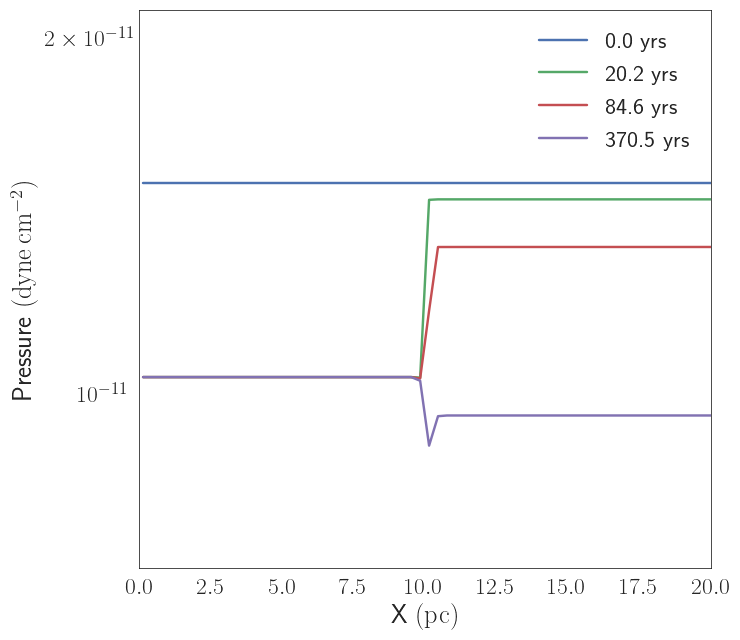
\includegraphics[width=1\linewidth]{DataImages/TabCoolingPRSprofile-micro}
	\caption{Το προφίλ της πίεσης ενός νέφους με ενεργοποιημένο το Tabulated Cooling Module κατά μήκος της ευθείας $y=0$ με το χρόνο, σε τάξη εκατοντάδων ετών.}
	\label{fig:tabcoolingprsprofile-micro}
\end{adjustwidth}
\end{figure}



	

	\subsubsection{Crossing Time}
	Ο σκοπός μας είναι να εξετάζουμε βήμα - βήμα τη δυναμική των νεφών. Παρότι εντοπίσαμε το παραπάνω σφάλμα, το οποίο θα προσπαθήσουμε να λύσουμε με την εφαρμογή διαφορετικών modules ψύξης, θα εξετάσουμε ακόμα μια παράμετρο του γενικού μας προβλήματος.
	
	 Από την εξίσωσης της ορμής:
	\begin{equation}
	\dv{\va V}{t}=-\frac{\grad P}{\rho}
	\end{equation}
	η διαφορά πίεσης που εμφανίζεται λόγο διαφορετικού ρυθμού (και κυρίως τερματισμού της) ψύξης των δύο αερίων δημιουργεί μια δύναμη προς τα έξω. Αποτέλεσμα αυτής της διαδικασίας είναι η διαστολή του νέφους. Ουσιαστικά η διαστολή αυτή είναι η μετάδοση δύο κυμάτων. Ενός κύματος συμπύκνωσης προς το εξωτερικό το οποίο συνοδεύεται από ένα κύμα αραίωσης στο εσωτερικό. Δηλαδή εν τέλει έχουμε μια φαινομενική "κατάρρευση" του νέφους, αφού η φαινομενική ακτίνα του (δηλαδή η ακτίνα εκείνη που διατηρεί την αρχική πυκνότητα) μικραίνει.
	 
	Η ταχύτητα διάδοσης αυτής της "κατάρρευσης" δηλαδή η ταχύτητα διάδοσης των δύο κυμάτων είναι η ταχύτητα του ήχου στο εκάστοτε μέσο. Η τοπική ταχύτητα του ήχου είναι:
	\begin{equation}
	c_s=\sqrt{\gamma \frac{P}{\rho}}
	\end{equation}
	όπου $\gamma = 5/3$
	
	
	Από τις αρχικές συνθήκες (παράγραφος~\ref{par:InitialConditions}) οι τοπικές ταχύτητες του ήχου για το εσωτερικό και το εξωτερικό είναι:
	\begin{align}
	c_s &=\SI{1.2}{km.s^{-1}} \qq{(MC)} \\
	c_s &=\SI{38.7}{km.s^{-1}} \qq{(ISM)}
	\end{align}
	
	Καθώς η πίεση πέφτει, η ταχύτητα του ήχου στο νέφος μειώνεται κατά ένα παράγοντα $\sim 0.75^{1/2}=0.8$ δηλαδή περίπου $1\si{.km.s^{-1}}$.
	
	\begin{marginfigure}
		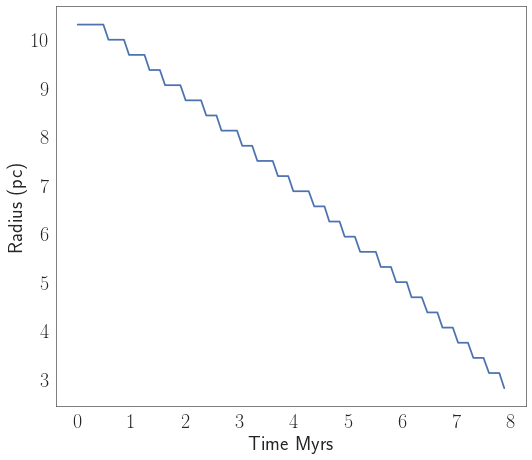
\includegraphics[width=1\linewidth]{DataImages/TabCoolingRadius}
		\caption{Εκτίμηση της ακτίνας του νέφους συναρτήσει του χρόνου. Υπολογίστηκε με βάση τη παράγωγο του προφίλ της πυκνότητας κατά μήκος της ευθείας $y=0$}
		\label{fig:tabcoolingradius}
	\end{marginfigure}
	
	Άρα τώρα μπορούμε να εκτιμήσουμε τη χρονική κλίμακα της "κατάρρευσης" με βάση την ακτίνα του νέφους:
	\begin{equation}
	\tau_R=\frac{R}{c_s} \simeq \SI{7.5}{\mega yrs}
	\end{equation}
	το οποίο φαίνεται να συμφωνεί με τη παρατήρηση, βλέπε σχήμα~\ref{fig:tabcoolingradius}.
	
	\subsubsection{Πρώτα Συμπεράσματα}
	Με τη χρήση του Tabulated Cooling Module του PLUTO δείξαμε ότι η προσπάθεια εξομοίωσης της δυναμική ενός σχετικά κρύου αερίου είναι εσφαλμένη καθώς οδηγεί σε μια κατώτατη θερμοκρασία η οποία προκύπτει από τα όρια του πίνακα θερμοκρασιών.
	
	Παρότι θα μπορούσαμε να επεκτείνουμε μέσω τεχνικών παρεμβολής τον πίνακα  $\Lambda (T)$ κρίναμε ότι κάτι τέτοιο απλά θα προσφέρει μια νέα χαμηλότερη θερμοκρασία και άρα μια επανάληψη των ίδιων περίπου αποτελεσμάτων με μια σχετική χρονική καθυστέρηση. 
	
	Άρα χρειαζόμαστε μια νέα προσέγγιση του όρου ψύξης στις χαμηλές θερμοκρασίες ώστε να αποκομίσουμε μια ρεαλιστικότερη απεικόνιση της εξέλιξης ενός κρύου αερίου μέσα στο διαγαλαξιακό μέσο.  
	
	Με βάση ένα εσφαλμένο μοντέλο έχουμε ενδείξεις για το πόσο σημαντικό ρόλο παίζει, σε νέφη τεραστίων διαστάσεων η ψύξη στις πολύ μικρές θερμοκρασίες. 
	
	\subsection{SNEq Cooling}
	Με βάση τα παραπάνω θα εξετάσουμε το δεύτερο module ψύξης μέσω ακτινοβολίας οπτικά αραιού μέσου του PLUTO, το οποίο ονομάζεται \textbf{Simplified Non-Equilibrium Cooling (SNEq)}. 
	
	Για να χρησιμοποιήσουμε το SNEq θα πρέπει να ορίσουμε σαν μια ακόμη μεταβλητή την
	αναλογία ουδετέρου Υδρογόνου σε σχέση με το Πλάσμα.
	Σε κάθε βήμα της εξομοίωσης ο κώδικας ολοκληρώνει μαζί με τις υδροδυναμικές εξισώσεις και την χρονική μεταβολή του $x_{H_I}$ μέσω της εξίσωσης:
	\begin{equation}
	\pdv{x_{\ce{HI}}}{t}=n_e \left( -(c_r+c_i)f_n+c_r\right) 
	\end{equation}
	μαζί με την εξίσωση της ενέργειας ή οποία γίνεται:
	\begin{equation}
	\pdv{t}(\rho e)=-\Lambda=-n_e n_H \left( \sum\limits_{k=1}^{16}j_k +w_{i/r} \right) 
	\end{equation}
	
	όπου η άθροιση στα $k$ υπολογίζει 16 διαφορετικές γραμμές εκπομπής 
	(Ly α, H α, HeI (584+623), CI (9850 + 9823), CII (156μ), CII (2325Å), NI (5200 Å),
	NII (6584 + 6548 Å), OI (63μ), OI (6300 + 6363 Å), OII (3727), MgII (2800), SiII (35μ), SII (6717 + 6727),FeII (25μ), FeII (1.6μ))
	\todo{Render line emmisions}
	
	Ο συντελεστής $j_k$ έχει μονάδες $\si{erg/sec . cm^3}$ και υπολογίζεται από τη σχέση:
	\begin{equation}
	j_k=\frac{\hbar^2 \sqrt{2\pi}}{\sqrt{k_B m_e}m_e}f_k q_{12}\frac{h \nu _k}{1+n_e (q_{21}/A_{21})}
	\end{equation}
	με $k$ τον δείκτη της εκάστοτε μετάπτωσης και $f_k=n_k/n_H$ το ποσοστό του εκάστοτε στοιχείου.
	\begin{align}
	q_{12}=\frac{\num{8.6e-6}}{\sqrt{T}}\frac{\Omega _{12}}{g_1}e^{-\frac{h\nu _k}{k_B T}} 
	&&
	q_{21}=\frac{\num{8.6e-6}}{\sqrt{T}}\frac{\Omega _{21}}{g_2}
	\end{align} 
	με $\Omega _{12} = \Omega _{21}$ η ισχύς της σύγκρουσης με τιμές οι οποίες είναι καταγεγραμμένες σε πίνακα.
	Το $w_{i/r}$ αντιπροσωπεύει τη θερμική ενέργεια που χάνεται από τον ιονισμό και την επανασύνδεση:
	\begin{equation}
	w_{i/r} = c_i\times \num{13.6}\times \num{1.6e-12} f_n +c_r \times \num{0.67}\times \num{1.6e-12} (1-f_n) \frac{T}{11590}
	\end{equation}
	όπου $c_r$ και $c_i$ είναι οι ρυθμοί ιονισμού και επανασύστασης του Υδρογόνου:
	\begin{align}
	c_r=\frac{\num{2.6e-11}}{\sqrt{T}} 
	&& 
	c_i=\frac{\num{1.08e-8}\sqrt{T}}{\num{13.6}^2} e^{-\frac{\num{157890}}{\sqrt{T}}}
	\end{align}
	
	
	\subsubsection{Εξομοίωση με SNEq Cooling}
	
	\begin{figure}[h]
		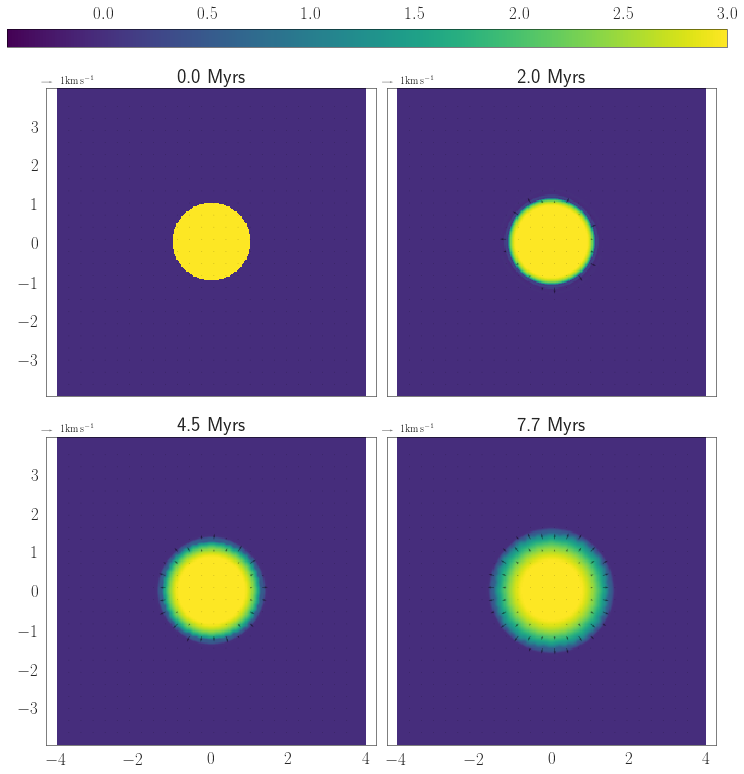
\includegraphics[width=0.7\linewidth]{DataImages/SNCoolingRHOquad}
		\caption{Ο χάρτης της πυκνότητας του νέφους στο χρόνο (σε λογαριθμική κλίμακα).}
		\label{fig:sncoolingrhoquad}
	\end{figure}
	
	\begin{marginfigure}
		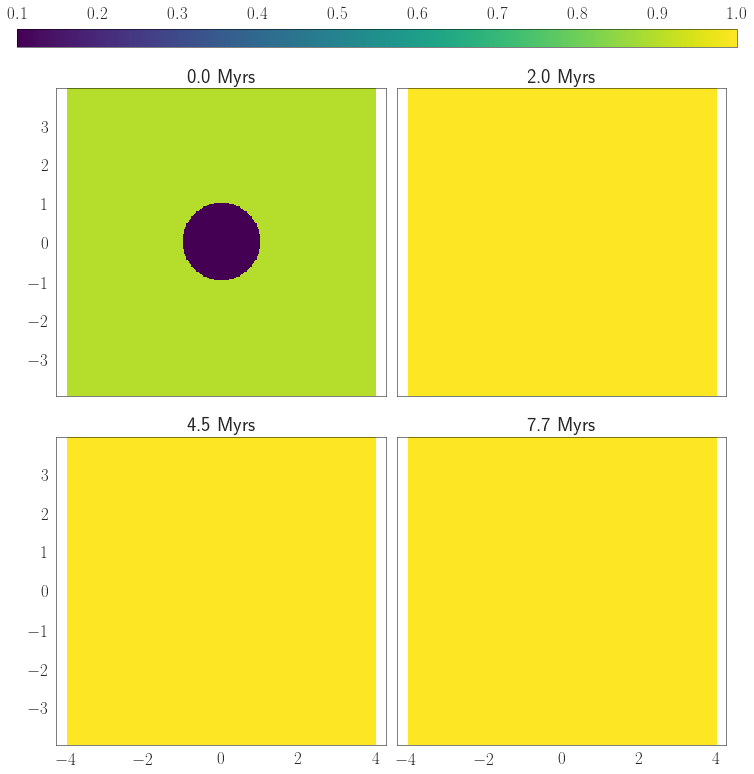
\includegraphics[width=1\linewidth]{DataImages/SNCoolingXHIquad}
		\caption{Χρονική εξέλιξη του ποσοστού ιονισμένου Υδρογόνου}
		\label{fig:sncoolingxhiquad}
	\end{marginfigure}
	
	
	Δεχόμενοι σαν βάση τη προηγούμενη προσπάθεια μας και τις ίδιες αρχικές συνθήκες για να χρησιμοποιήσουμε το SNEq Cooling Module θα πρέπει να ορίσουμε το ποσοστό ουδετέρου Υδρογόνου $x_{H_I}$.
	\todo{Τα παρακάτω είναι λάθος, ΞΑΝΑ}
	Θεωρώντας οτι το κρύο νέφος έχει μικρότερο ποσοστό ιονισμένου Υδρογόνου χρησιμοποιούμε τη τιμή $x_{H_I}=0.1$ εντός του νέφους και $x_{H_I}=0.9$ 
	στο μεσοαστρικό χώρο.
	
\begin{figure}[h]
	\begin{adjustwidth}{-5cm}{-0cm}
	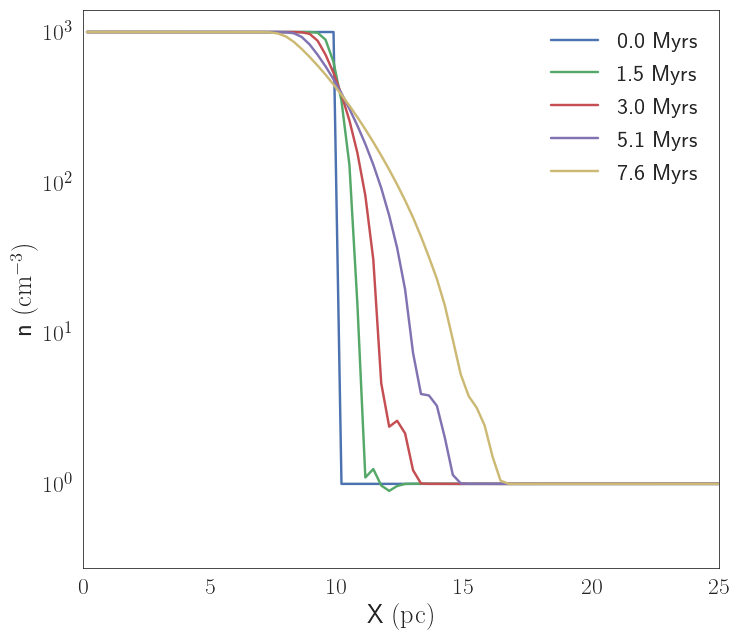
\includegraphics[width=1\linewidth]{DataImages/SNCoolingRHOprofile}
	\caption{Το προφίλ της πυκνότητας του αερίου με ενεργοποιημένο το SNEq Cooling Module κατά μήκος της ευθείας $y=0$ με το χρόνο.}
	\label{fig:sncoolingrhoprofile}
\end{adjustwidth}
\end{figure}

\begin{figure}[h]
	\begin{adjustwidth}{-5cm}{-0cm}	
	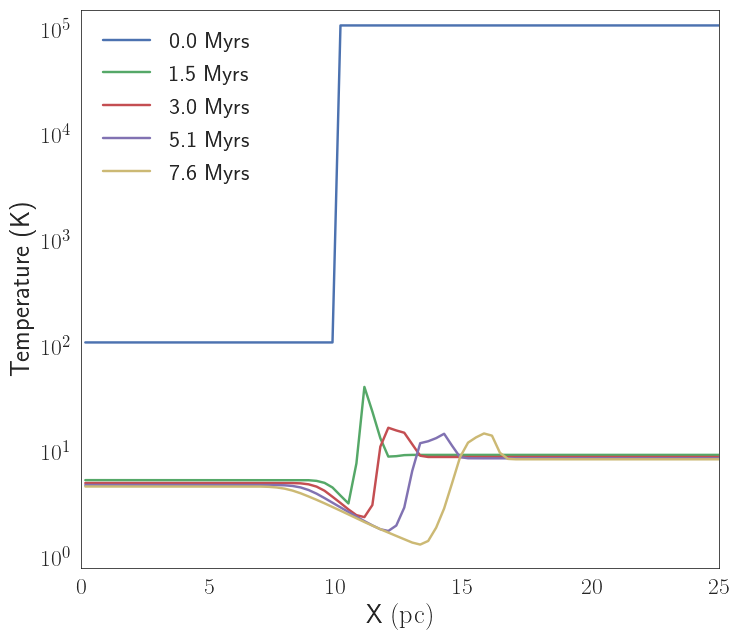
\includegraphics[width=1\linewidth]{DataImages/SNCoolingTMPprofile}
	\caption{Το προφίλ της θερμοκρασίας του αερίου με ενεργοποιημένο το SNEq Cooling Module κατά μήκος της ευθείας $y=0$ με το χρόνο.}
	\label{fig:sncoolingtmpprofile}
\end{adjustwidth}
\end{figure}

Η θερμοκρασία του νέφους φτάνει σε τίμες κάτω των $\SI{10}{K}$ το οποίο συμφωνεί με τα παρατηρησιακά δεδομένα από τα μοριακά νέφη (\ref{fig:sncoolingtmpprofile}).

Η διαφορά πίεσης με το περιβάλλον είναι κατά μία τάξη μεγέθους μικρότερη σε σχέση με τη περίπτωση του Tabulated Cooling, με αποτέλεσμα μια μικρότερη επιτάχυνση του ρευστού προς τα έξω (σχήμα \ref{fig:difftabcoolsncoolprsprofile-edit}).


\begin{figure}[h]
	\begin{adjustwidth}{-0cm}{-5cm}	
	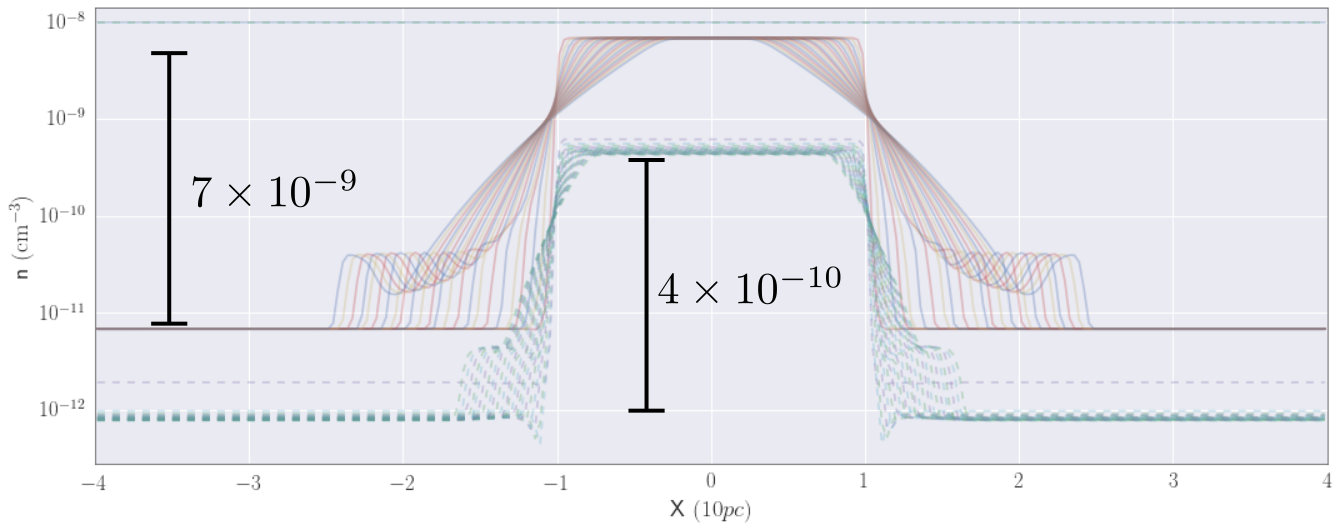
\includegraphics[width=1\linewidth]{DataImages/diffTabCoolSNCoolPRSprofile-edit}
\caption{Το προφίλ της πίεσης του αερίου με ενεργοποιημένο το SNEq Cooling Module (διακεκομένη γραμμή) σε σύγκριση με αυτή του Tabulated Cooling κατά μήκος της ευθείας $y=0$ με το χρόνο.}
\label{fig:difftabcoolsncoolprsprofile-edit}
\end{adjustwidth}
\end{figure}
Τα σχετικά αποτελέσματα που φαίνονται στα παρακάτω σχήματα μας δείχουν οτι σε μια crossing time ($\sim \SI{8}{Myrs}$) το μεγαλύτερο μέρος του νέφους είναι άθικτο (\ref{fig:sncoolingrhoprofile},\ref{fig:sncoolingrhoquad}).  \todo[inline]{γιατι άραγε?} 


Παρότι έχουμε σαφώς καλύτερα αποτελέσματα σε σχέση με το προηγούμενο Cooling Module του PLUTO, η τελική εικόνα δεν είναι ρεαλιστική καθώς όπως βλέπουμε από το σχήμα~\ref{fig:sncoolingxhiquad} με το ποσοστό του $x_{H_I}$ το νέφος δείχνει ιονισμένο \todo[inline]{?????}

\newpage
	\subsection{H2 Cooling}
	Η ψύξη μέσω του SNEq είχε εμφανώς καλύτερα, δηλαδή πιο ρεαλιστικά αποτελέσματα αλλά διατηρεί ένα μεγάλο πρόβλημα που έχουμε για τις χαμηλές θερμοκρασίες. Οι μαγνητουδροδυναμικοί αριθμητικοί κώδικες αντιλαμβάνονται το ρευστό σαν ιονισμένο πλάσμα. Παρότι σε μεγάλες θερμοκρασίες η προσέγγιση αυτή είναι καλή σε χαμηλές θερμοκρασίες εμφανίζονται ουδέτερα άτομα και μόρια.
	
	Το SNEq module μέσω του χειρισμού του ποσοστού $x_{H_I}$ έκανε ένα βήμα προς αυτή τη κατεύθυνση αλλά για ένα μοριακό νέφος με μεγάλες ποσότητες σε \ce{H_2}, πληθώρα άλλων μορίων (\ce{He}, \ce{CO} κλπ) μαζί με σκόνη προφανώς η προσέγγιση αυτή δεν είναι αρκετή.
	
	Έτσι δοκιμάσαμε και το επόμενο Cooling Module που διαθέτει ο PLUTO το οποίο ονομάζεται \textbf{Molecular Hydrogen Non-Equilibrium Cooling (H2 COOL)}.
	
	Το H2COOL εισάγει με τη σειρά του 2 ακόμα μεταβλητές. Έτσι, εκτός του ποσοστού ουδετέρου υδρογόνου, έχουμε το ποσοστό ιονισμένου υδρογόνου $x_{H_{II}}$ και το ποσοστό μοριακού Υδρογόνου $x_{H_2}$.
	\begin{align}
	x_{H_I} =\frac{n_{H_I}}{n_H} && x_{H_I} =\frac{n_{H_{II}}}{n_H} && x_{H_2} =\frac{n_{H_2}}{n_H} 
	\end{align}
	όπου η συνολική αριθμητική πυκνότητα του Υδρογόνου $n_H=n_{H_I}+n_{H_{II}}+2n_{H_2}$.
	
	Η χημική εξέλιξη του μοριακού, ατομικού και ιονισμένου υδρογόνου ακολουθεί τις αντιδράσεις:
	\begin{align}
	&\ce{H + e^- -> H^+ + 2e^-} && k_1 = \num{5.84e-11} \sqrt{T} e^{\num{-157809}/T} \\
	&\ce{H^+ + e^- -> H + h\nu} && k_2 = \num{2.6e-11} \sqrt{T}\\
	&\ce{H_2 + e^- -> 2H + e^-} && k_3 = \num{4.4e-10}T^{0.35} e^{\num{-102000}/T}\\
	&\ce{H_2 + H -> 3H} && k_4=\num{1.067e-10}T_{eV}^{2.012} e^{\frac{\num{-4.463}}{T_{eV}}(1+\num{0.2472}T_{eV})^{3.512}}\\
	&\ce{H_2 + H_2 -> H_2 + 2H} && k_5=\num{1.0e-8}e^{-\num{84100}/T} \\
	&\ce{H + H ->[dust] H_2} && k_6=\num{3.0e-17}\sqrt{T_2} (1+0.4\sqrt{T_2}+0.2 T_2 +0.08 (T_2)^2)
	\end{align}
	όπου $T$ η θερμοκρασία σε Κέλβιν, $T_{eV}$ η θερμοκρασία σε ηλεκτρονιοβόλτ, $T_2=\frac{T}{100}$ και $k_i$ ο ρυθμός εξέλιξης της κάθε αντίδρασης σε $\si{cm^3 s^{-1}}$.
	
	Η εξέλιξη των αριθμητικών πυκνοτήτων υπολογίζεται από την εξίσωση:
	\begin{equation}
	S_i=\dv{n_i}{t}=\sum\limits_{j,k}k_{j,k}n_j n_k - n_i \sum_{j}k_{i,j}n_j
	\end{equation}
	\todo{Δεν είμαι σίγουρος οτι είναι ακρβωςο όρος $S_i$ }
	όπου $k_{j,k}$ είναι ο ρυθμός παραγωγής του $i$ στοιχείου από τα υπόλοιπα στοιχεία $j$ και $k$, και $k_{i,j}$ ο ρυθμός καταστροφής του $i$ στοιχείου από όλα τα $j$ στοιχεία.
	
	Ο κώδικας ολοκληρώνει τα ποσοστά των 3 ειδών υδρογόνου μέσω της επίλυσης της παραπάνω εξίσωσης μαζί με την εξίσωση μεταφοράς:
	\begin{equation}
	\pdv{X_i}{t}=-\va{u}\cdot \grad{X_i}+S_i
	\end{equation}
	όπου ο όρος μεταφοράς $-\va{u}\cdot \grad{X_i}$ ολοκληρώνεται μαζί με τις υδροδυναμικές εξισώσεις μάζας, ορμής (hydro step) ενώ ο όρος $S_i$ ολοκληρώνεται κατά το βήμα της ψύξης (cooling step).
	
	Οι ενεργειακές απώλειες λόγω ψύξης τελικά υπολογίζονται, εκτός από τις παραπάνω αντιδράσεις, από τις απώλειες ιονισμού λόγω κρούσης $\Lambda _{\mathtt{CI}}$ και επανασύνδεσης λόγω ακτινοβολίας $\Lambda _{\mathtt{RR}}$, απώλειες λόγω περιστροφής και ταλάντωσης (rotational-vibrational cooling) $\Lambda _{\mathtt{rotvib}}$ και διάσπασης (dissosiation) $\Lambda _{\mathtt{diss}}$ των μορίων \ce{H_2}, και της διαδικασίας αλληλεπίδρασης σκόνης-αερίου (gas-grain process) $\Lambda _{\mathtt{grain}}$.
	\begin{equation}
	\Lambda = \Lambda _{\mathtt{CI}} + \Lambda _{\mathtt{RR}} +\Lambda _{\mathtt{rotvib}} + \Lambda _{\mathtt{diss}} + \Lambda _{\mathtt{grain}}
	\end{equation}
	
	\todo[inline]{Depending on the requirement, the user can add more components to the cooling function, for e.g., cooling due to fixed fractions of standard molecules like CO, OH, H 2 O etc or contributions from collisional excitation of lines as indicated in the SNEq module.}

	\begin{marginfigure}
	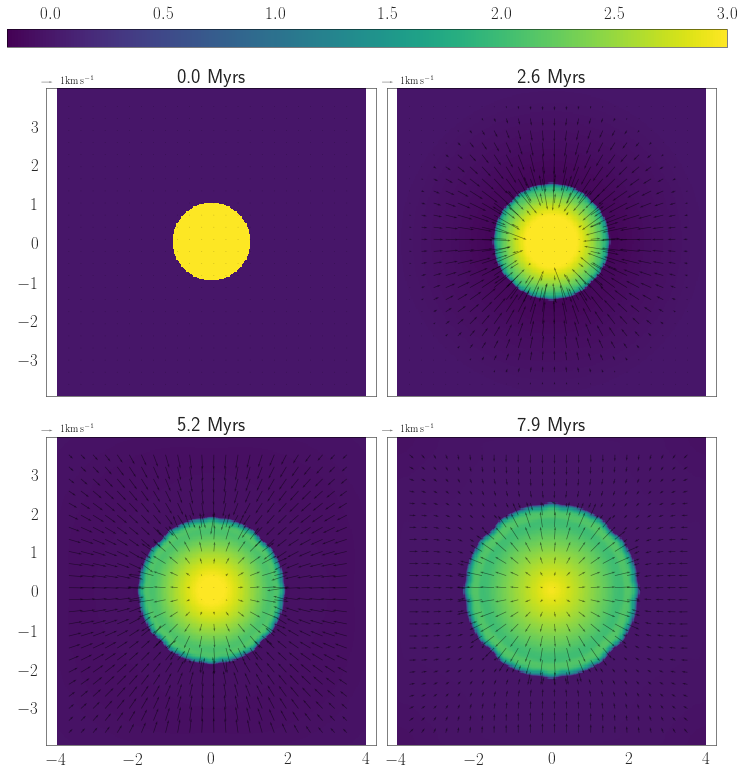
\includegraphics[width=1.\linewidth]{DataImages/H2CoolingRHOquad}
	\caption{Η πυκνότητα του αερίου σε διάφορες χρονικές στιγμές}
	\label{fig:h2coolingrhoquad}
\end{marginfigure}	

	\subsubsection{Εξομοίωση με H2COOL}
		\marginpar{
		\begin{table}[H]
			\caption{Αρχικές συνθήκες για τα ποσοστά των διαφορετικών μορφών Υδρογόνου}
			\label{tab:h2sc}
			\begin{tabular}{|l|  c |  c| c|}
				\toprule
				Περιοχή & $x_{\ce{H_Ι}}$ & $x_{\ce{H_{ΙΙ}}}$ & $x_{\ce{H_2}}$ \\ 
				\midrule
				Μοριακό Nέφος & $0.1$ & $0$ & $0.9$ \\
				Μεσογαλαξιακό μέσο  & $0.9$ & $0.1$ & $0$ \\
				\bottomrule
			\end{tabular}
		\end{table}
	}

	Ακολουθώντας την ίδια πορεία με προηγουμένως ορίζουμε στις αρχικές συνθήκες τα ποσοστά μοριακού, ουδετέρου και ιονισμένου υδρογόνου όπως φαίνονται στο πίνακα~\ref{tab:h2sc}.


	Το πρώτο που παρατηρούμε είναι ότι το νέφος διαστέλλεται σε χρονική κλίμακα τάξης του crossing time. Ο λόγος είναι γιατί η διαφορά πιέσεων είναι πολύ μεγαλύτερη καθώς το κεντρικό τμήμα του νέφους διατηρεί τη πίεση στα ίδια επίπεδα με την αρχική πίεση $10^{-8}$. Για να αλλάξει η πυκνότητα στο εσωτερικό του νέφους χρειάζεται ενάς αρκετά μεγαλος χρόνος, άρα η σχετική στασιμότητα της πίεσης σημαίνει και στασιμότητα της θερμοκρασίας. Όντως όπως βλέπουμε και στο σχήμα~\ref{fig:h2coolingtmpprofile} η θερμοκρασία του νέφους διατηρείται κοντά 
στην αρχική τιμή των $\SI{100}{K}$.

	Ενώ για το διαγαλαξιακό μέσο ο ρυθμός ψύξης φαίνεται να επιβραδύνεται αρκετά κοντά στους $\SI{3e3}{K}$ καθώς ολόκληρο το υδρογόνο μετατρέπεται σε ουδέτερο (σχήμα \ref).
\todo[inline]{Καθώς το υδρογονο επανασυνδεεται HII -> HI ολοκληρη η ενεργεια παει εκει και δεν ψυχεται}

\begin{figure}[h]
	\begin{adjustwidth}{-0cm}{-5cm}
	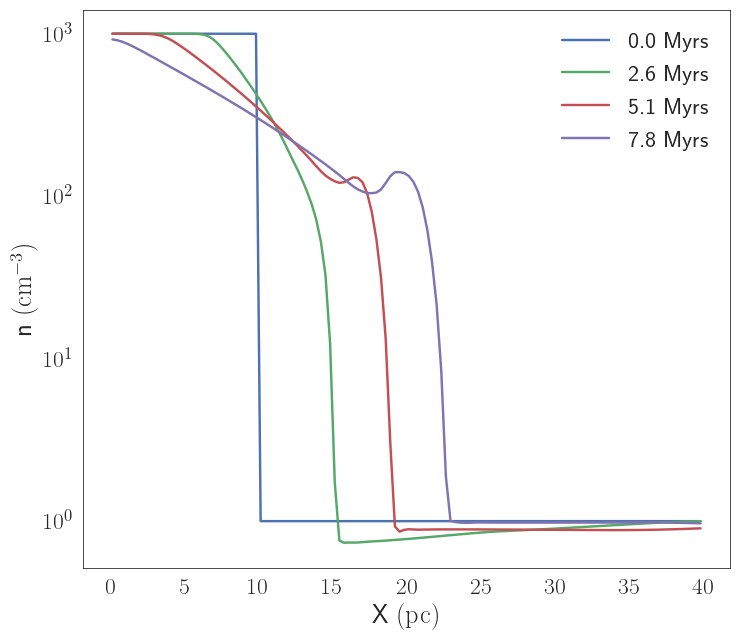
\includegraphics[width=1\linewidth]{DataImages/H2CoolingRHOprofile}
	\caption{Το προφίλ της πυκνότητας του αερίου με ενεργοποιημένο το Η2 Cooling Module κατά μήκος της ευθείας $y=0$ με το χρόνο.}
	\label{fig:h2coolingrhoprofile}
	\end{adjustwidth}
\end{figure}


\begin{figure}[h]
	\begin{adjustwidth}{-5cm}{-0cm}
	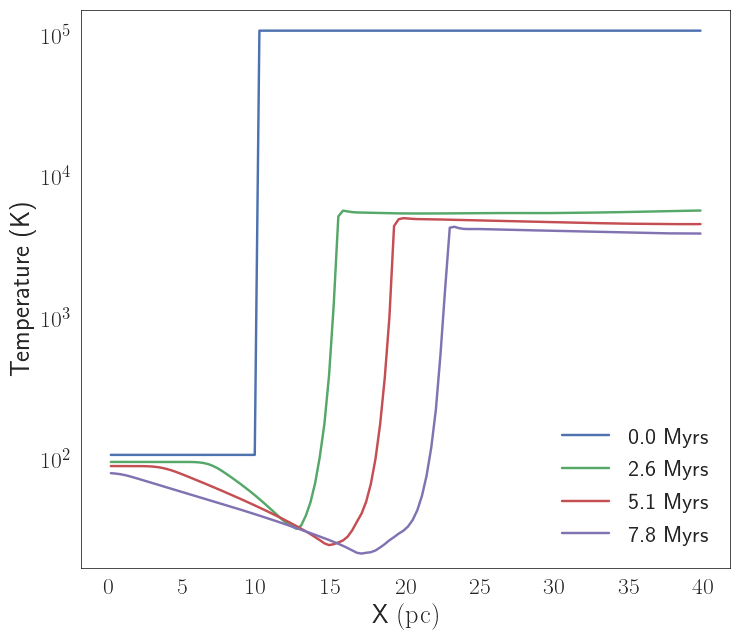
\includegraphics[width=1\linewidth]{DataImages/H2CoolingTMPprofile}
	\caption{Το προφίλ της θερμοκρασίας του αερίου με ενεργοποιημένο το Η2 Cooling Module κατά μήκος της ευθείας $y=0$ με το χρόνο.Με διακεκομμένες γραμμές και στα ίδια χρονικά στιγμιότυπα το ποσοστό ουδετέρου υδρογόνου.}
	\label{fig:h2coolingtmpprofile}
	\end{adjustwidth}
\end{figure}



\begin{figure}[h]
	\begin{adjustwidth}{-5cm}{-0cm}
	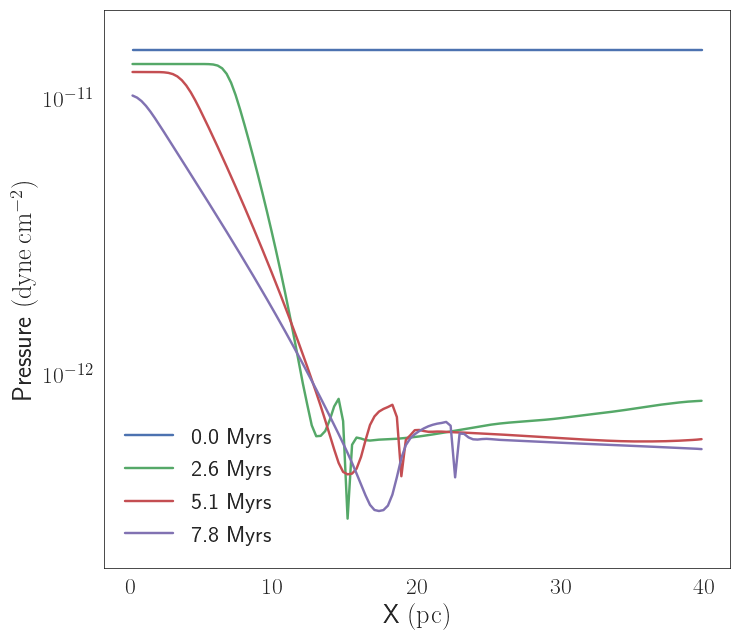
\includegraphics[width=1\linewidth]{DataImages/H2CoolingPRSprofile}
	\caption{Το προφίλ της πίεσης του αερίου με ενεργοποιημένο το Η2 Cooling Module κατά μήκος της ευθείας $y=0$ με το χρόνο.}
	\label{fig:h2coolingprsprofile}
	\end{adjustwidth}
\end{figure}

	

	
	Οι παρατηρήσεις των μοριακών νεφών μας δίνουν θερμοκρασίες της τάξεως των $\SI{30}{K}$. Η ασυμφωνία με την εξομοίωση μπορεί αν εξηγηθεί με βάση δύο παρατηρήσεις:
	\begin{itemize}
		\item Χρησιμοποιήσαμε μια αρχική θερμοκρασία των $\SI{100}{K}$ θεωρώντας αυταπόδεικτο ότι αυτή θα μειωθεί μέχρι το παρατηρούμενο νούμερο. Ειδάλλως αν χρησιμοποιούσαμε σαν αρχική θερμοκρασία τους $\SI{30}{K}$ μπορεί να διατηρούταν σε αυτή. Γι αυτό το λόγο χρησιμοποιούμε μια διαφορετική θερμοκρασία έτσι ώστε να μην "επιβάλλουμε" το δικό μας αποτέλεσμα.
		\item Το module H2COOL απευθύνεται αυστηρά στις μεταβάσεις και μεταβολές του Υδρογόνου. Σύμφωνα με \todo{τεκμηρίωση} όμως η ενεργειακές μεταβάσεις του Υδρογόνου παύουν να είναι σημαντικές σε χαμηλότερες των $\SI{100}{K}$ όπου κυρίαρχο ρόλο παίζουν τα \ce{CO}, \ce{OH}, \ce{H_2 O} και ίσως και το \ce{He}.
	\end{itemize}
	

	\subsection{MINEQ Cooling}
	\todo[inline]{Δεν έχω κάνει ακόμα τις εξομοιώσεις, πολλες οι μεταβλητες}
	
	\newpage
	\section{Βαρύτητα}
	Είναι προφανές ότι έναν από τους ισχυρότερους ρόλους στην αστροφυσική (αν όχι το μεγαλύτερο) τον παίζει η βαρύτητα. 
	
	
	
	
	The second add in our simulation is Gravity. \todo{Add momentum equation with Gravity}
	\subsection{Self Gravity}
	\label{par:SolidSphereSelfGravit}
	Επειδή ο PLUTO δεν μπορεί να χειριστεί την ιδιοβαρύτητα θα προσπαθήσουμε να τη προσεγγίσουμε τοποθετώντας ένα βαρυτικό δυναμικό ομογενούς σφαίρας στο εσωτερικό του νέφους και ένα δυναμικό σημειακής μάζας στο εξωτερικό του νέφους. Δηλαδή:
	\begin{equation}
		\vec{g}(x,y) = 
		\begin{cases}
			\frac{GM}{R^3}(x \vu x+ y \vu y) &\texttt{if } r<R \\
			\frac{GM}{r^3}(x \vu x+ y \vu y) &\texttt{if } r>R
		\end{cases}
	\end{equation}
	
	όπου $r=\sqrt{x^2+y^2}$
	
	\subsubsection{Βαρυτική Σταθερά}
	Για να χρησιμοποιήσουμε τη δύναμη της βαρύτητας θα πρέπει να υπολογίσουμε τη σταθερά $G$ σε μονάδες κώδικα, όπως βλέπουμε και από το πίνακα~\ref{tab:cd}. Άρα 
	\begin{equation}
		G=G_\texttt{cgs} \si{cm^3.g^{-1}.s^{-2}} = G_\texttt{cgs} \frac{\SI{1.67e-24}{g.cm^{-3}}}{\rho_0}\frac{10^{18}\si{s^2}}{t^2_0}
	\end{equation}
	Αντικαθιστώντας $G_\texttt{cgs}=\SI{6.674e-8}{}$ βρίσκουμε
	\begin{equation}
		\boxed{G=\SI{1.114e-13}{G_0}}
	\end{equation}
	όπου $G_0=(\rho_0 t_0)^{-1}$ η σταθερά της βαρύτητας σε μονάδες κώδικα.
	
%	\begin{marginfigure}
%		\includegraphics[width=1.0\linewidth]{astro/Diplomatiki/logDensityG}
%		\caption{Density Simulation (Logarithmic Scale) over four different times in one $t_\texttt{ff}$.}
%		\label{fig:logdensityg}
%	\end{marginfigure}
	
	\subsubsection{Χρόνος Ελεύθερης Πτώσης}
	Ο χρόνος ελεύθερης πτώσης (free-fall time) είναι η χρονική κλίμακα που χρειάζεται ένα σώμα να καταρρεύσει κάτω από το ίδιο το βάρος του, αν δεν υπεισέρχονται άλλες δυνάμεις που να αντισταθμίσουν ή να επιταχύνουν τη διαδικασία. Έτσι παίζει ένα πολύ σημαντικό ρόλο στις χρονικές κλίμακες πολλών αστροφυσικών διεργασιών.
	
	Στη περίπτωση του δικού μας νέφους ο χρόνος ελεύθερης πτώσης υπολογίζεται:
	\begin{equation}
		t_\texttt{ff}=\sqrt{\frac{3\pi}{32G\rho}} = \SI{51404}{t_0} = \SI{1.6}{Myrs}
	\end{equation}
	
	Για να εξετάσουμε την επίδραση της βαρύτητας αρχικά θα εκτελέσουμε την εξομοίωση που έχουμε κάνει και προηγουμένως, αρχικά σε ένα νέφος που δεν εμπεριέχει διαδικασία ψύξης.
	
\begin{figure}[h]
	\begin{adjustwidth}{-5cm}{-0cm}
	\centering
	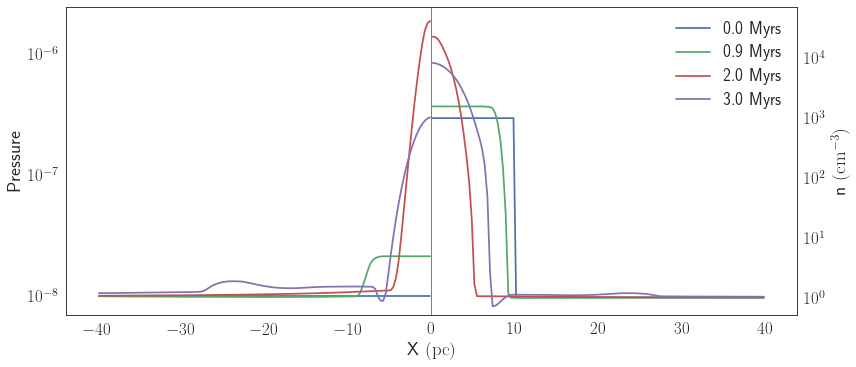
\includegraphics[width=1\linewidth]{DataImages/NoCoolGRHOprofile}
	\caption{Το προφίλ της πυκνότητας του αερίου μέσα σε βαρυτικό δυναμικό ομογενούς σφαίρας κατά μήκος της ευθείας $y=0$ με το χρόνο.}
	\label{fig:nocoolgrhoprofile}
	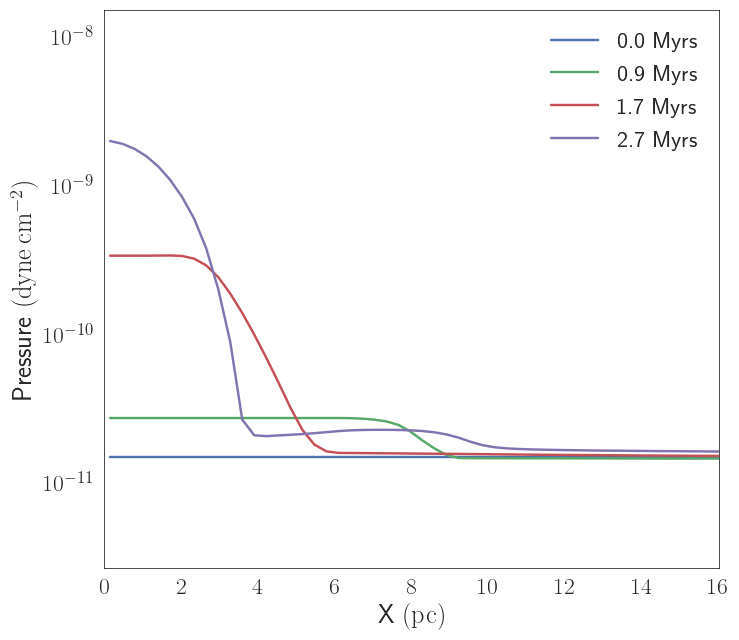
\includegraphics[width=1\linewidth]{DataImages/NoCoolGPRSprofile}
	\caption{Το προφίλ της πίεσης του αερίου μέσα σε βαρυτικό δυναμικό ομογενούς σφαίρας κατά μήκος της ευθείας $y=0$ με το χρόνο.}
	\label{fig:nocoolgprsprofile}
\end{adjustwidth}
\end{figure}

Το αποτέλεσμα όπως φαίνεται από το σχήμα~\ref{fig:nocoolgrhoprofile} δείχνουν ένα χρόνο κατάρρευσης κοντά στα $\SI{2}{Myrs}$ καθώς στη συνέχεια το νέφος αναπηδά λόγω της θερμικής πίεσης (σχήμα~\ref{fig:nocoolgprsprofile}) και επιταχύνεται προς τα έξω.
Το αποτέλεσμα είναι πολύ κοντά στην τιμή του χρόνου ελεύθερης πτώσης καθώς η πίεση δεν ήταν αρκετή για να επιβραδύνει νωρίτερα την κατάρρευση και επίσης η ακρίβεια των εξομοιώσεων δεν είναι αρκετή για να διαχειρίστει απόλυτα σωστά το φαίνομενο της βαρυτικής κατάρρευσης. Ένα pixel αντιστοιχεί σε $\SI{0.3125}{parsec}\simeq \SI{1}{ly}$ μέγεθος πολύ μεγαλύτερο από ένα πρωτοαστέρα.

\subsubsection{Σφαιρικό νέφος με Radiation Cooling με ιδιοβαρύτητα}

Θεωρώντας μέχρι στιγμής το πιο ρεαλιστικό προσομοιωτή ψύξης αυτό του H2COOL, θα δοκιμάσουμε να επαναλάβουμε τη προσομοίωση μέσα σε δυναμικό ιδιοβαρύτητας έτσι όπως ορίστηκε στη παράγραφο~\ref{par:SolidSphereSelfGravit}. 
%
%	\subsubsection{Jeans Radius} 
%	\todo[inline]{λάθος ο υπολογισμός}
%	From the momentum equation we can estimate a critical Radius of a solid cloud by solving the equation:
%	\begin{equation}
%		\frac{\grad P}{\rho}=\frac{GM}{R^3}r 
%	\end{equation}
%	Where we can make an order of magnitude estimation:
%	\begin{equation}
%		\frac{P}{r^* \rho}=\frac{GM}{R^3}r^* \rightarrow \boxed{r^*=\left( \frac{PR^3}{G\rho ^2}\right) ^{1/5}}
%	\end{equation}
%	
%	For our cloud this calculation gives a critical radius of $\SI{4.6}{pc}$
%	
	
	\subsubsection{Σφαίρα Bonnor-Ebert}
	Η σφαίρα Bonnor-Ebert είναι η θεωρητική κατασκευή μιας ισόθερμης σφαίρας όπου η βαρύτητα εξισορροπείται από την εσωτερική πίεση. Δηλαδή ισχύουν οι εξισώσεις:
	\begin{align}
	\frac{Gm}{r^2} &+\frac{1}{\rho}\frac{dP}{dr}=0 \text{ Εξίσωση Κίνησης}\\
	\frac{dm}{dr} &= 4 \pi r^2 \rho \text{ Εξίσωση διατήρησης της Μάζας}\\
	P &= c_s ^2 \rho \text{ Καταστατική Εξίσωση}
	\end{align}
	
	Συνδυάζοντας και τις τρείς έχουμε:
	\begin{equation}
	\frac{1}{r^2}\frac{d}{dr} \left( r^2 c_s ^2 \frac{d \ln \rho}{dr}\right)  = -4 \pi G \rho
	\end{equation}
	
	Η λύση της οποίας μας δίνει τη πυκνότητα συναρτήση της ακτίνας μέσα στο μοριακό πυρήνα:
	\begin{equation}
	\label{eq:B-E_density}
	\rho (r) =\frac{c_s ^2}{2 \pi G} \frac{1}{r^2}
	\end{equation}
	
	
	
	\section{Αλληλεπίδραση με Jet}
	Βασικός σκοπός της εργασίας μας είναι η μελέτη της αλληλεπίδρασης ενός jet με τα μοριακά νέφη του γαλαξία.
	
	
	
%	\nocite{*}
%	\printbibliography
\end{document}